%!TEX root = ms.tex
\clearpage
\begin{refsection}
%\renewcommand*{\thepage}{A\arabic{page}}
\beginsupplement
\appendix
\pagenumbering{arabic}
\begin{center}
\textbf{\large Supplemental Material: \\ On the usage of rank percentile in evaluating and predicting the scientific impact}

Sen Tian, Panos Ipeirotis
\end{center}

\section{Rank percentile indicators for scholars}
\label{sec:suppl_similarity_autrp}

We consider the benchmark being the area of biology. In order to study the agreement of various indicators, for each indicator, we classify the scholars into four classes, class $1$: $0\le \text{S}_m^{ib}(t) < 0.25$, class $2$: $0.25\le \text{S}_m^{ib}(t) < 0.5$, class $3$: $0.5 \le \text{S}_m^{ib}(t) < 0.75$ and class $4$: $0.75 \le \text{S}_m^{ib}(t) \le 1$. An agreement is when two (or three) different indicators belong to the same class. The overall agreement for all three indicators, S$_{P5}$, S$_c$, and S$_h$, is $51\%$ at age $5$ and $68\%$ at age $30$; that is, for about half of the scholars the three indicators agree with each other at age $5$, while that number becomes around two third at age $30$. Figure \ref{fig:aut_rp_class} displays pairwise agreement of the three indicators. We see that the agreement increases with the age. Furthermore, S$_{P5}$ has large agreement with both S$_{c}$ and S$_{h}$, which are $69\%$ and $67\%$, respectively, at age $5$, and $71\%$ and $81\%$, respectively, at age $30$. 

Figure \ref{fig:hm_autrp_current} shows the correlation between S$_c^{ib}(t_1)$ and S$_c^{ib}(t_2)$, and the correlation between S$_h^{ib}(t_1)$ and S$_h^{ib}(t_1)$. The magnitudes of correlations are similar to those for S$_{P5}$ as shown in Figure \ref{fig:hm_rp_aut}.

% fig:aut_rp_class
% class agreement among all the author rp
\begin{figure}[ht!]
    \centering
    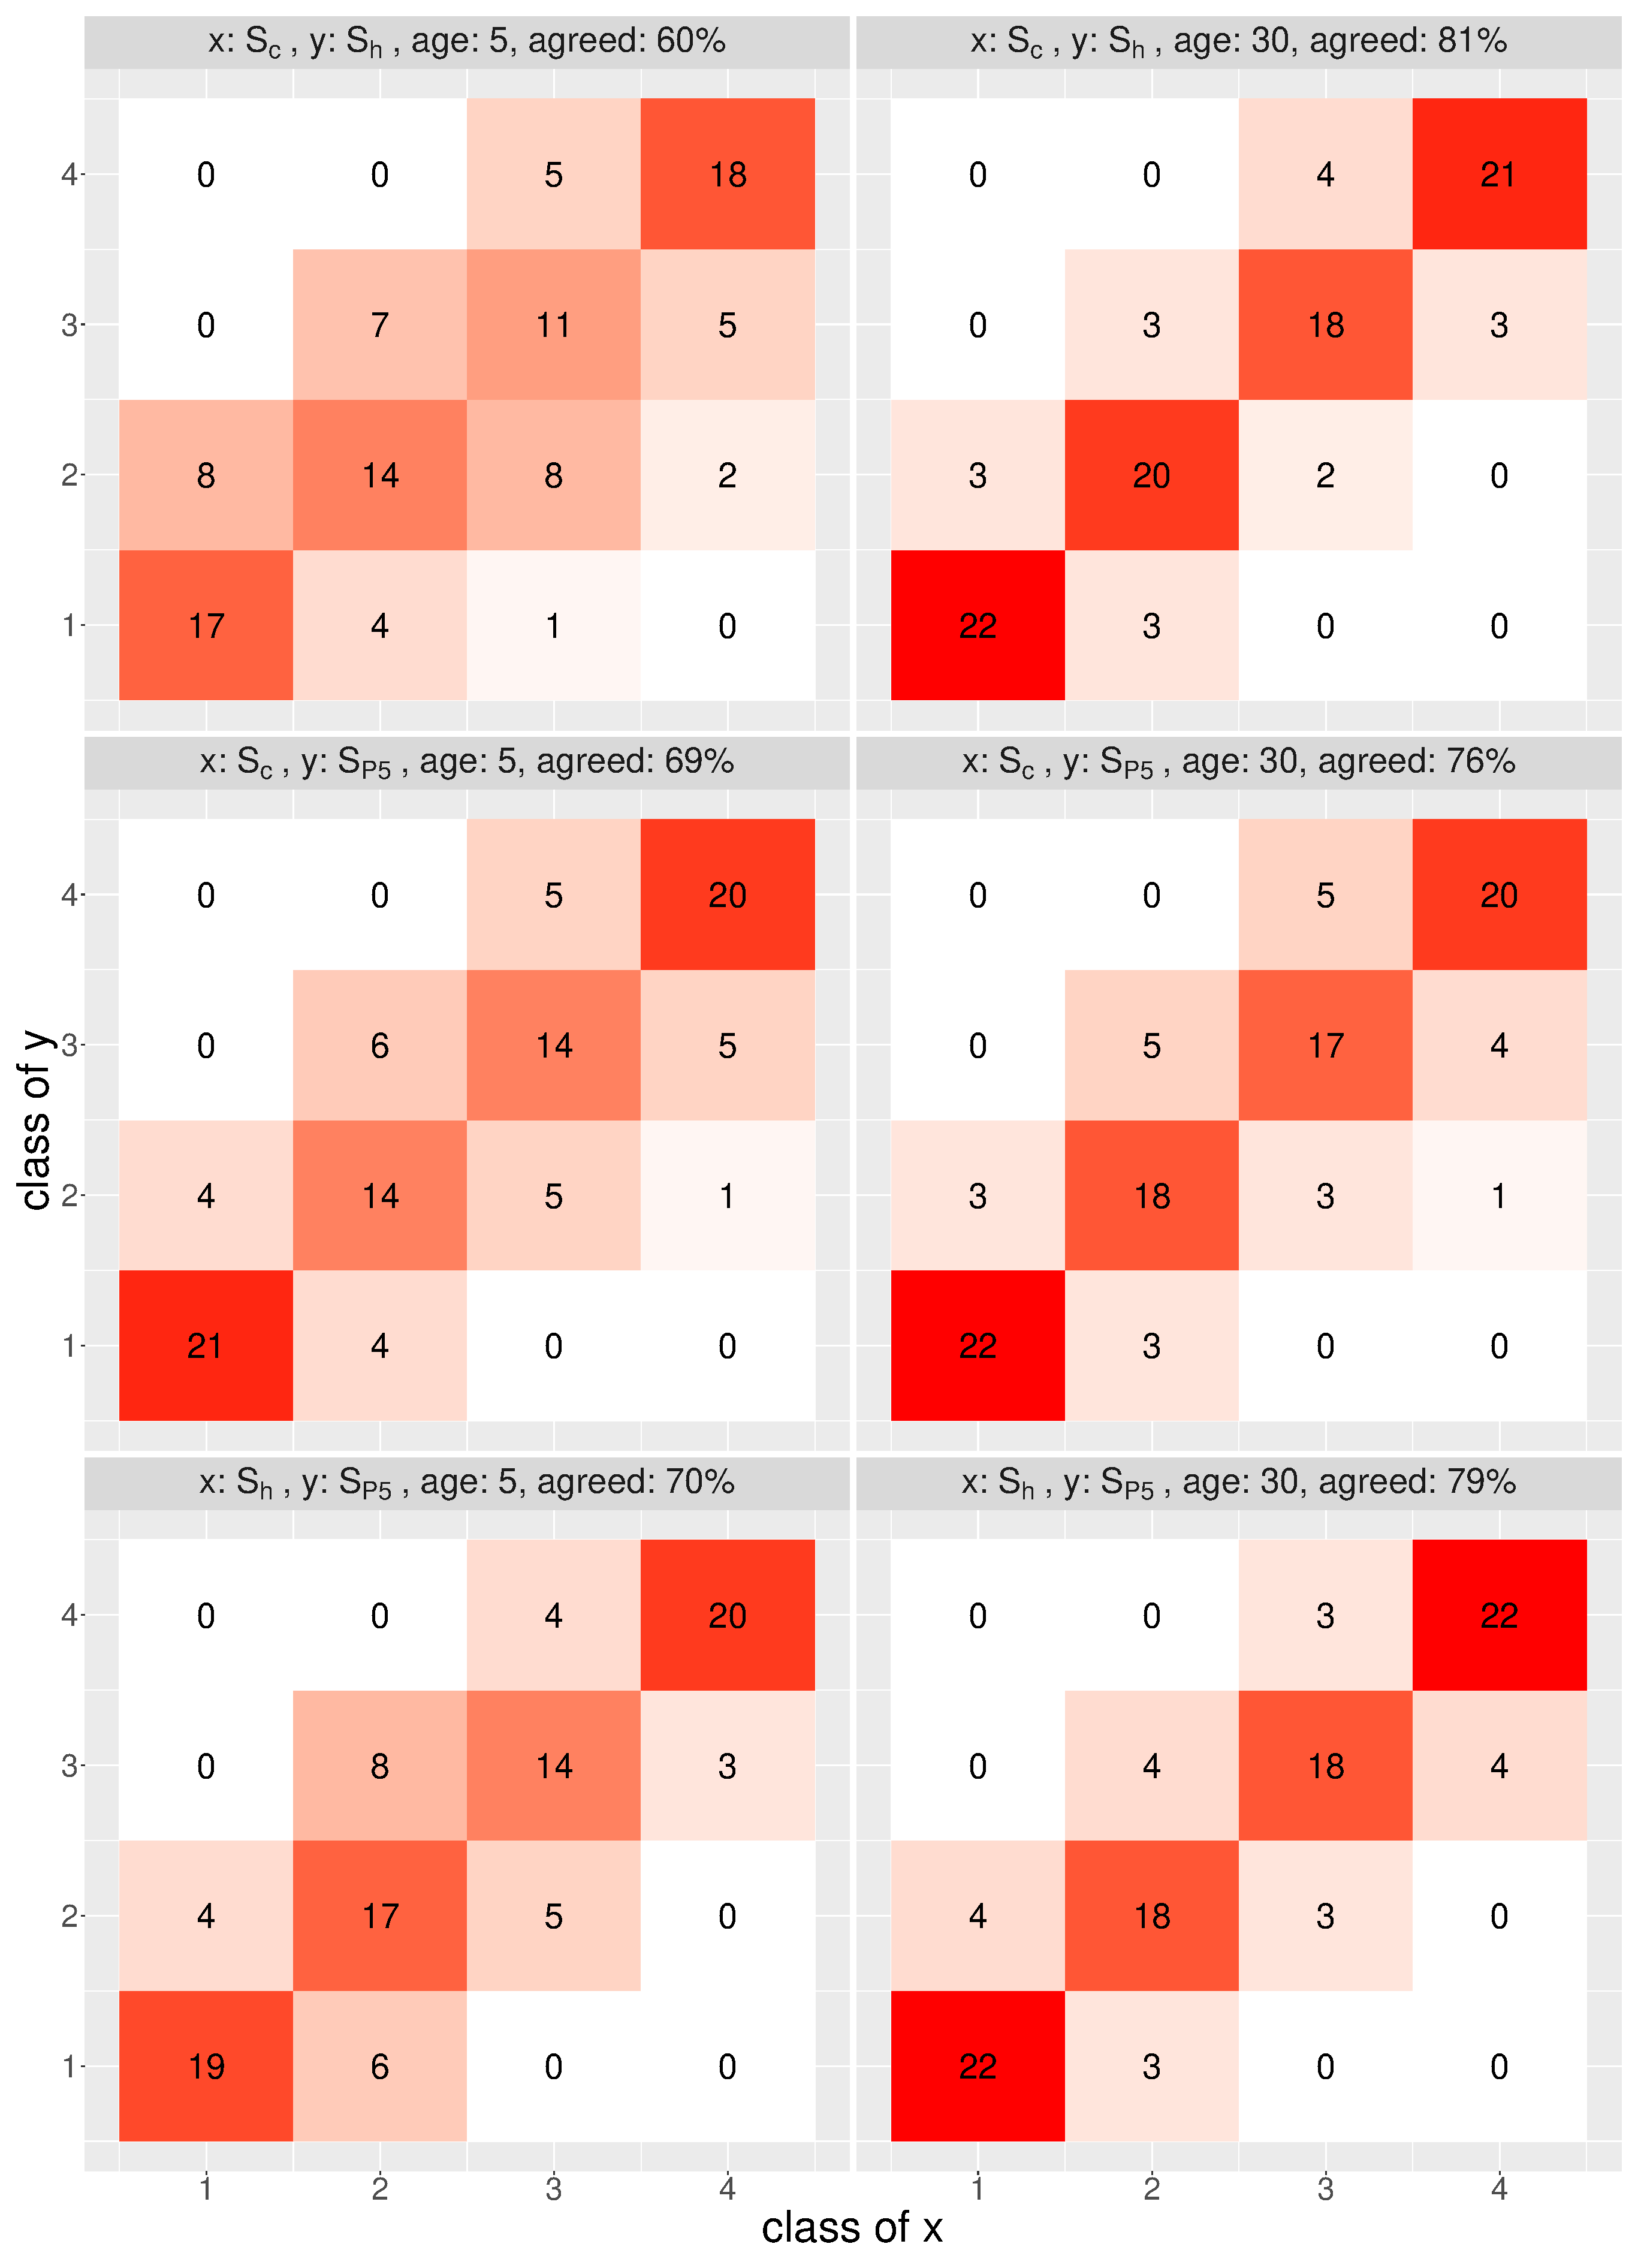
\includegraphics[width=0.88\textwidth]{figures/compare_autrp/heatmap_class_agreement.eps}
    \caption[The agreement of rank percentile indicators for scholars]{Rank percentile indicators are classified into four groups, that are class $1$: $0 \le \text{S}_m^{ib}(t) < 0.25$, class $2$: $0.25 \le \text{S}_m^{ib}(t) < 0.5$, class $3$: $0.5 \le \text{S}_m^{ib}(t) < 0.75$ and class $4$: $0.75 \le \text{S}_m^{ib}(t) \le 1$. The agreement of classes (sum of the anti-diagonal elements) is displayed in the title of each panel. The benchmark is biology. The agreement for all three indicators is $51 \%$ at age $5$ and is $68 \%$ at age $30$.}
    \label{fig:aut_rp_class}
\end{figure}

% publication rank percentile, heat map of correlations
\begin{figure}[ht!]
    \centering
    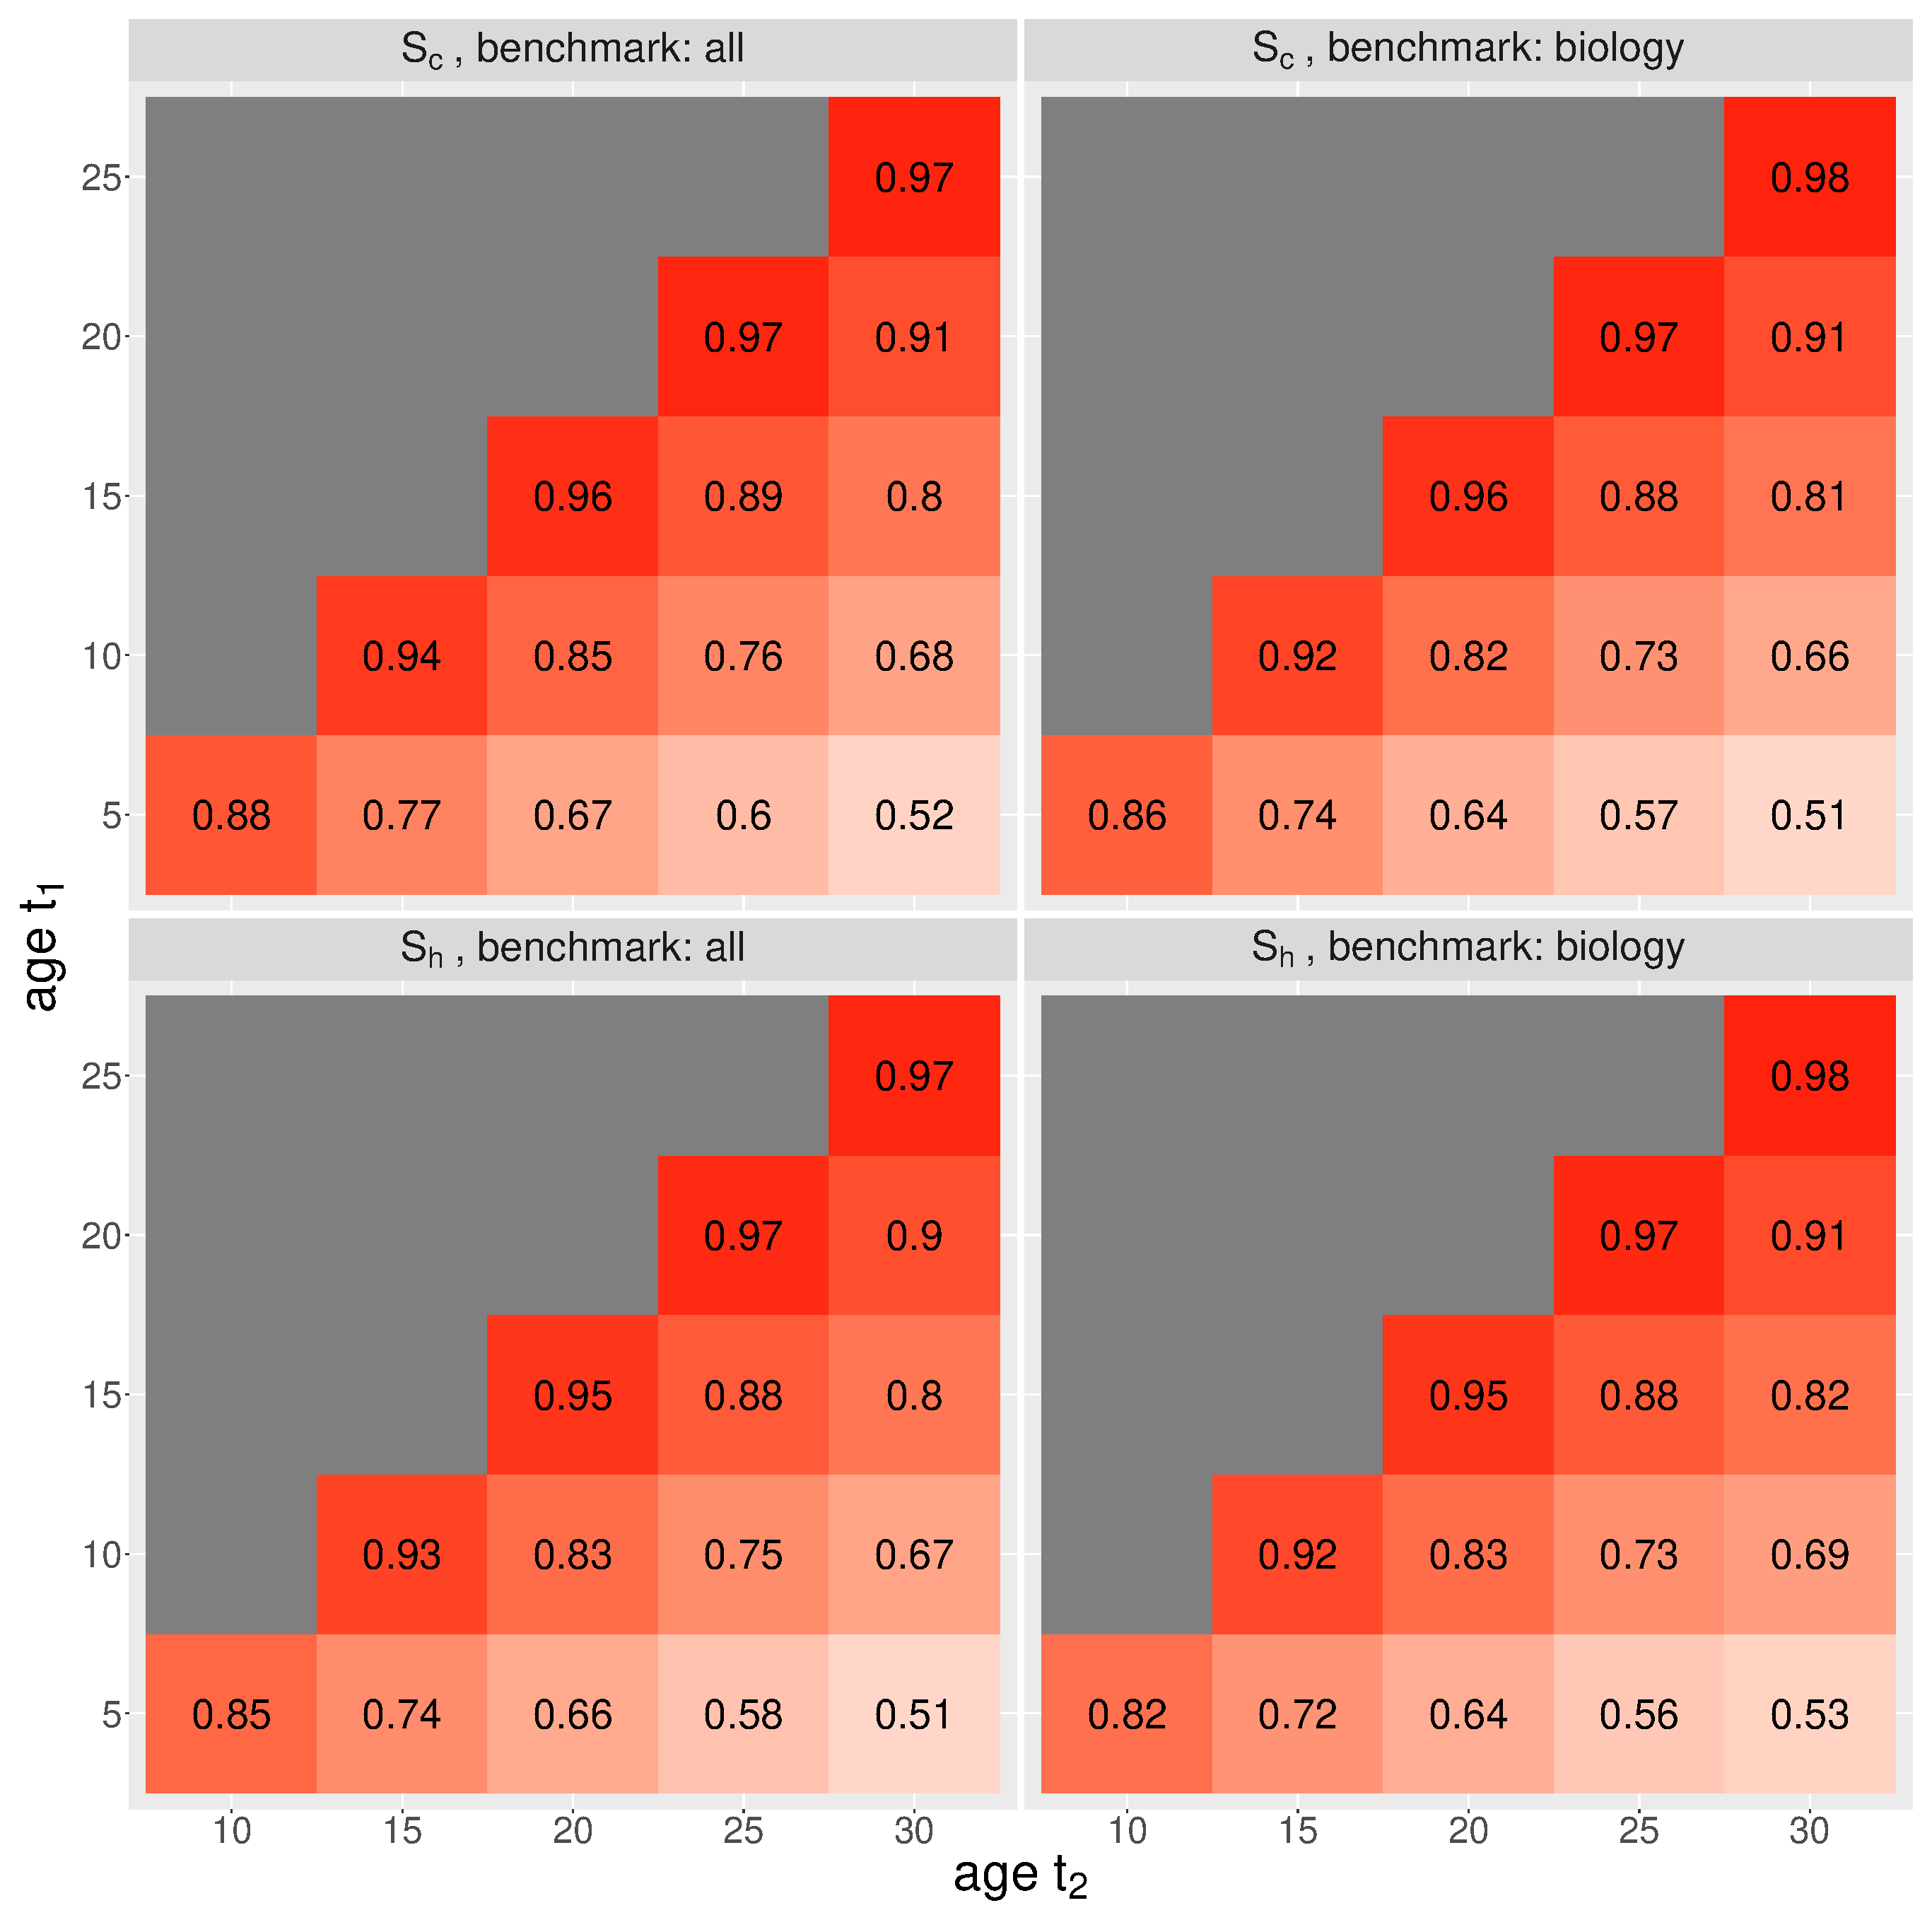
\includegraphics[width=\textwidth]{figures/pred_power/suppl_heatmap_cor_current.eps}
    \caption[Correlation heatmap for S$_c$ and S$_h$.]{The Pearson's correlation between rank percentile indicators at two different ages. }
    \label{fig:hm_autrp_current}
\end{figure}



\section{Robustness of \texorpdfstring{S$_{P5}$}{Lg}}
\label{sec:suppl_robustness_P5}

Recall that S$_{P5}^{ib}(t)$ is calculated based on an aggregation of the performances of publications that scholar $i$ publishes by age $t$. Denote $\text{m}_{P5}^{ib}(t)$ as the evaluation metric of scholar $i$ at age $t$ based on $\text{P}_{c}^{jb}(5)$, that is $\text{m}_{P5}^{ib}(t)= \sum_{j=1}^{N(t)} \text{P}_{c}^{jb}(5)$, where $N(t)$ is the total number of publications of scholar $i$ by age $t$. We illustrated in the paper that P$_c$ exhibits high stability, and hence P$_{c}^{jb}(5)$ can be applied to represent the performance of the publication. 

We further demonstrate the robustness of S$_{P5}$ by considering a longer citation history for each publication. Figure \ref{fig:robustness_test_cor} illustrates that m$_{P5}$ is highly correlated with m$_{P10}$ at age $t=1,\cdots,30$, where $\text{m}_{P10}^{ib}$t$= \sum_{j=1}^{N(t)} \text{P}_{c}^{jb}(10)$. We also consider the maximum, mean and median values of $\text{P}_{c}^{jb}(t)$, e.g. $\text{m}_{Pmax}^{ib}$t$= \sum_{j=1}^{N(t)} \max_{t^\prime}\text{P}_{c}^{jb}(t^\prime)$. We see from the figure that these metrics also exhibit high correlations with m$_{P5}$. Furthermore, we perform a Wilcoxon paired signed-rank test to compare the differences between S$_{P5}$ and S$_{P10}$ at each age $t=1,\cdots,30$, and the p-values are close to $1$; indicating that the differences are not statistically significant. Similar conclusions can be drawn for other indicators being considered.

\begin{figure}[ht!]
    \centering
    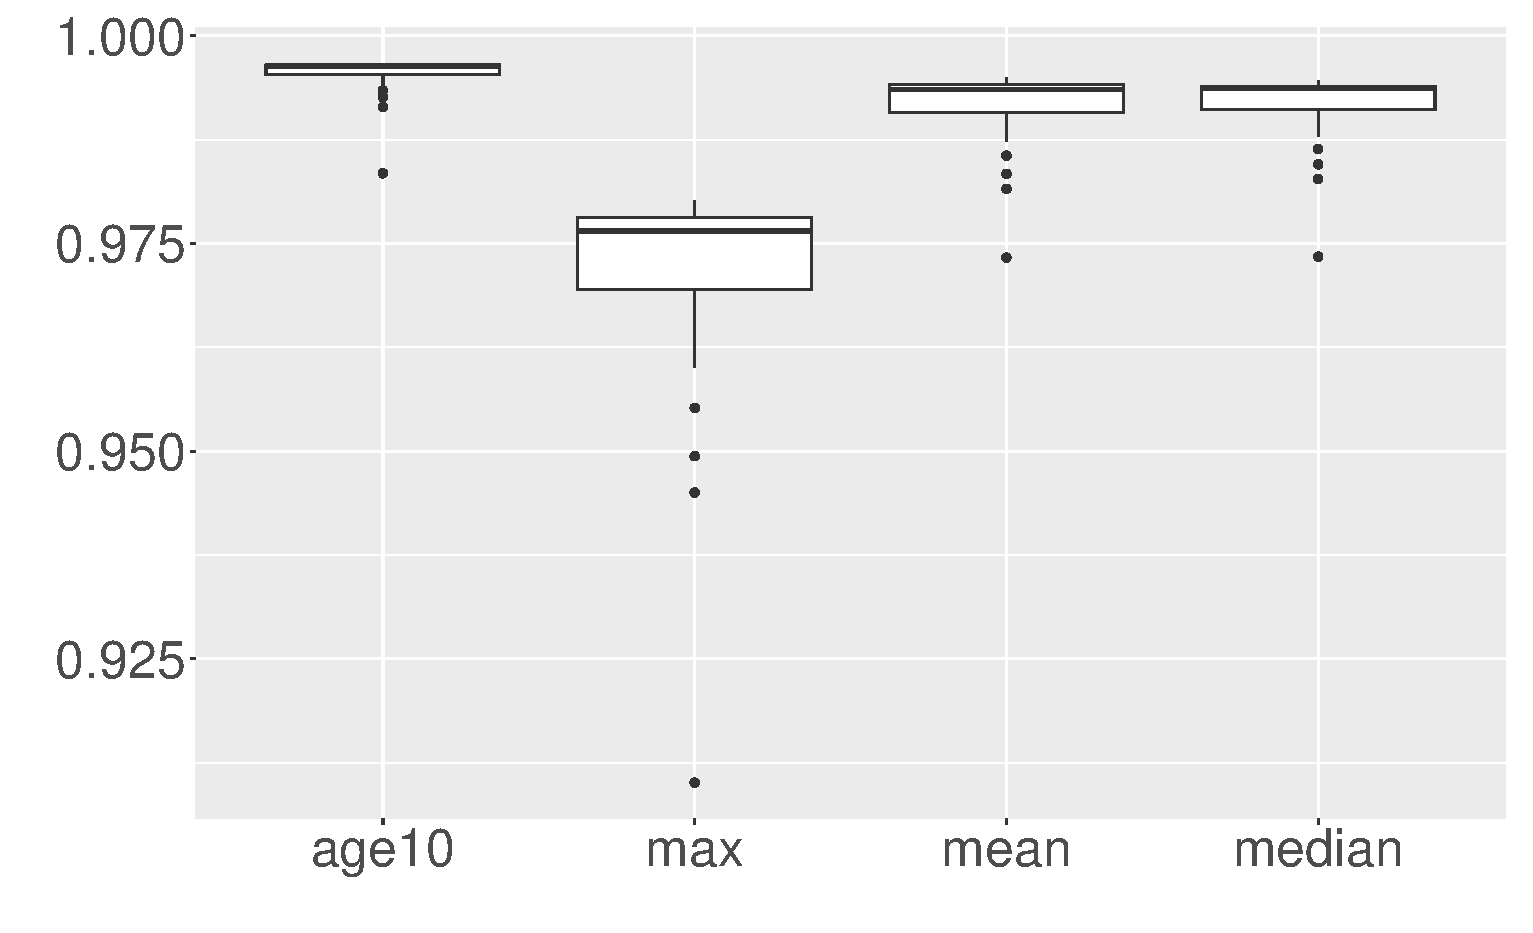
\includegraphics[width=0.7\textwidth]{figures/robustness/cor.eps}
    \caption[Correlation between m$_{P5}$ and other choices of evaluation metric]{Pearson's correlation between m$_{P5}$ and other choices of evaluation metric. Age $10$, max, mean and median correspond to m$_{P10}$, m$_{Pmax}$, m$_{Pmean}$ and m$_{Pmedian}$, respectively. The correlation is calculated at each age $t=1,\cdots,30$.}
    \label{fig:robustness_test_cor}
\end{figure}


\iffalse
\begin{equation}
\label{eq:rp_matrix}
\bordermatrix{
    & \text{age 1}     & \text{age 2}     & \cdots & \text{age $K$}     \cr
    \text{paper 1}     & \text{rp}_{11}^{(c)}     & \text{rp}_{12}^{(c)}     & \ldots & \text{rp}_{1 K}^{(c)}      \cr
    \text{paper 2}     & \text{rp}_{21}^{(c)}     & \text{rp}_{22}^{(c)}    & \ldots & \text{rp}_{2 K}^{(c)}     \cr
    \quad \vdots & \vdots & \vdots & \ddots & \vdots \cr
    \text{paper $N$}     & \text{rp}_{N 1}^{(c)}     & \text{rp}_{N 2}^{(c)}     & \ldots  & \text{rp}_{N K}^{(c)}    \cr
}
\end{equation}

We take the maximum performance for each of the $N$ papers, and sum them:
\begin{equation}
    \omega_{i \tau} = \sum_{j=1,\cdots,N} \max_{k=1,\cdots, K} \text{rp}_{j k} ^{(c)}.
\end{equation}
\fi

\section{Stationarity test}
\label{sec:suppl_stationarity}

Two commonly used statistical tests for stationarity are the Dicky-Fuller test~\cite{dickey1979distribution} and KPSS test~\cite{kwiatkowski1992testing}. These two tests formulate the hypothesis testing problems differently. Dicky-Fuller test assumes a unit root presented in the series. A unit root means that the series is $I(1)$, i.e. integrated order $1$ and the first differenced series is stationary. The more negative the test statistic is, the stronger the rejection of the null. On the other hand, KPSS test assumes the null as the series being stationary, i.e. $I(0)$. KPSS test is slightly more general since it allows testing a series being non-stationary but does not present a unit root. The more positive the test statistic is, the stronger the rejection of the null. Both tests include the drift in the test equations but exclude the trend, since we do not observe significant trends in the series. 

The test statistics are shown in Figure \ref{fig:stationarity_test}. The dashed lines indicate the critical values at $5 \%$ level. KPSS test indicates that P$_c$ and S$_{P5}$ are non-stationary series, and we do not have enough evidence to reject them being $I(1)$ according to the Dicky-Fuller test. Furthermore, the differenced series are stationary based on both tests.


\begin{figure}[ht!]
    \centering
    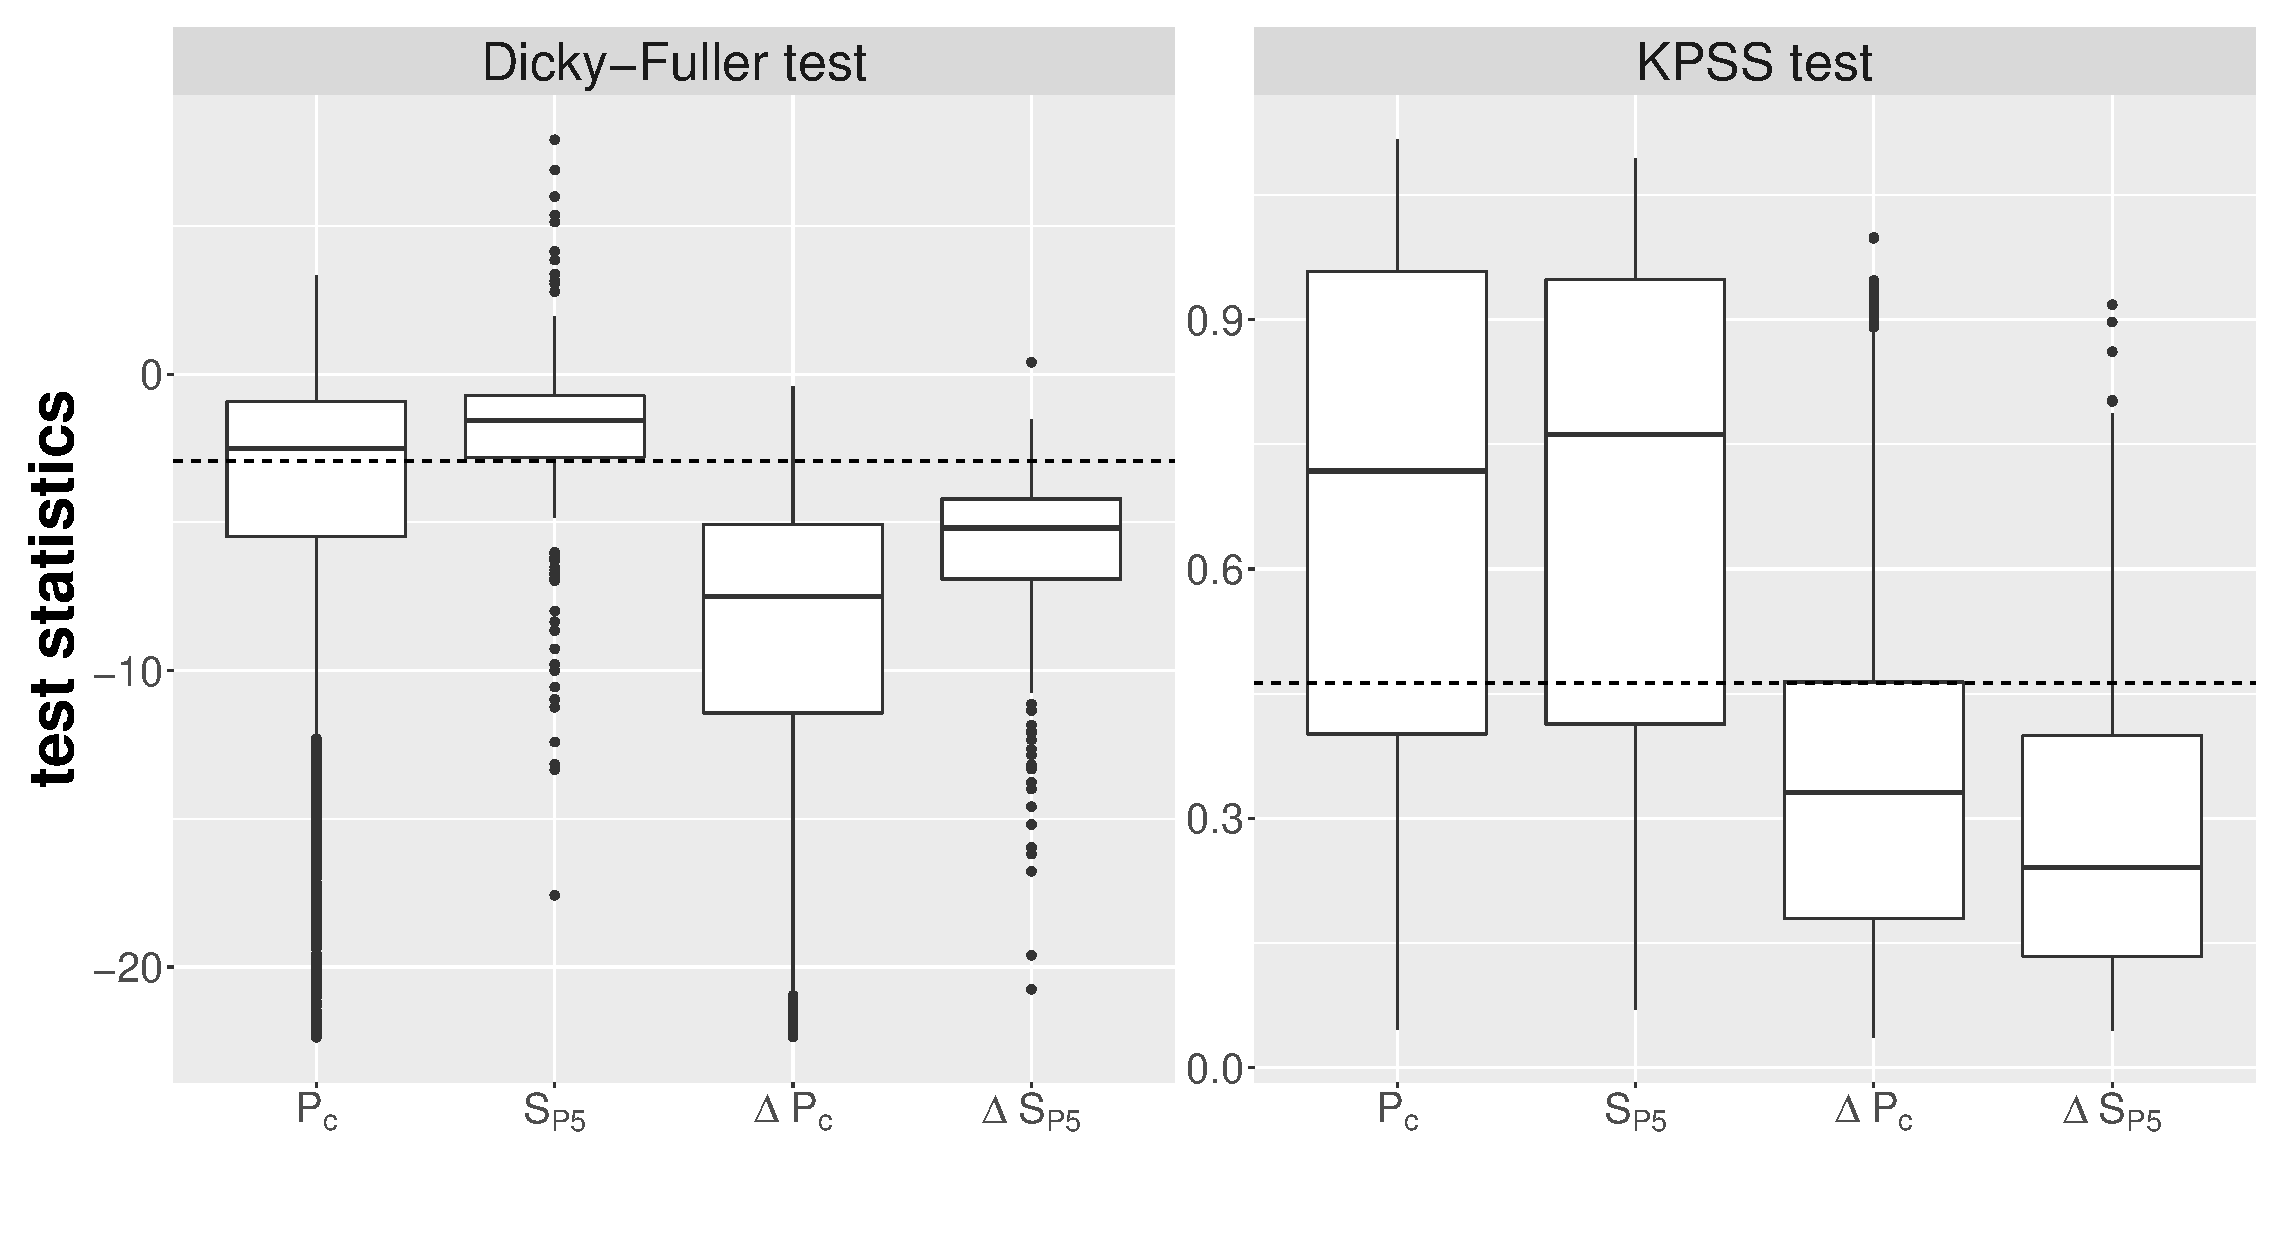
\includegraphics[width=\textwidth]{figures/stationarity/df_kpss.eps}
    \caption[Stationarity test of rank percentile series]{Statistical tests for the stationarity of rank percentile series. Both tests are applied on every individual series, and the test statistics are presented. The $5\%$ critical value for each test is illustrated by the dashed horizontal line. Both tests suggest that publication indicator P$_c$ and scholar indicator S$_{P5}$ are non-stationary, while their differenced series are stationary. }
    \label{fig:stationarity_test}
\end{figure}

\iffalse
\section{Details of the predictive models}
\label{sec:suppl_details_predmodel}

The details of the predictive models are described below.
\begin{itemize}
    \item Baseline: simple linear regression of P$_{it_2}^c$ on P$_{it_1}^c$. Same applies for S$_{it}^{P5}$.
    \item Simple Markov model (sm): linear regression of P$_{it_2}^c$ on P$_{it_1}^c$ and the change of P$_{it}^c$ over the last $2$ ages, i.e. P$_{it_1}^c$-P$_{it_1-2}^c$. Same applies for S$_{it}^{P5}$.
    \item Penalized linear regression models, including the ridge, lasso, elastic net (enet) and the Gamma lasso (gamlr): linear models with different penalties on the regression coefficients. All of these methods shrink the coefficients towards zero, and the later three methods can provide sparse solutions (shrink the coefficients to be exactly zeros). 
    \item Ensemble methods of regression trees, including the random forest (rf) and extreme gradient boosting trees (xgbtree): rf is a bagging of regression trees with a subset of randomly selected features chosen at each split to avoid overfitting. xgbtree is a fast implementation of gradient boosting on regression trees with a model formation that emphasizes the role of regularizations to avoid overfitting.
    %\item Support vector regression (svr)~\cite{drucker1997support}: 
    \item Neural networks (nnet): feedforward networks with multiple hidden layers, and using dropout and $l_2$ regularization to avoid overfitting.
\end{itemize}
\fi


\begin{table}[htbp]
  \centering
    \begin{tabular}{l|l}
    Method & Tuning parameters \\
    \midrule
    Lasso & Penalty strength parameter \\
    \midrule
    Ridge & Penalty strength parameter \\
    \midrule
    \multirow{2}[2]{*}{Elastic net} & Penalty strength parameter \\
          & Penalty gap parameter \\
    \midrule
    \multirow{2}[2]{*}{Gamma lasso} & Penalty strength parameter \\
          & Convexity parameter \\
    \midrule
    \multirow{3}[2]{*}{Random forest} & Number of trees to grow \\
          & Number of variables used at each split \\
          & Minimum number of observations in a node \\
    \midrule
    \multirow{9}[2]{*}{xgbtree} & Maximum number of iterations \\
          & Learning rate \\
          & Regularization parameter \\
          & Maximum depth of the tree \\
          & Minimum number of observations in each child leaf \\
          & Number of observations supplied to a tree \\
          & Number of features supplied to a tree \\
          & Regularization parameter for ridge penalty \\
          & Regularization parameter for LASSO penalty \\
    \midrule
    \multirow{5}[1]{*}{Deep neural network} & Number of layers  \\
          & Learning rate \\
          & Number of hidden units at each layer \\
          & Dropout rate \\
          & Regularization parameter \\
    \end{tabular}%
  \caption[Hyperparameter(s) of the machine learning models]{Hyperparameter(s) of the machine learning models.}
  \label{tab:hyperpara}%
\end{table}%

\begin{table}[htbp]
  \centering
    \begin{tabular}{l|l}
    Feature & Description \\
    \midrule
    pub\_cit\_cumulative & total citations of publication $j$ \\
    pub\_cit\_yearly & yearly citations of publication $j$ received in $t_1$ \\
    pub\_cit\_peryear & average citations of publication $j$ over age \\
    pub\_rp\_cumulative & rank percentile indicator calculated based on total citations, i.e. P$_c^{jb}(t_1)$ \\
    pub\_rp\_yearly & rank percentile indicator calculated based on yearly citations at $t_1$\\
          &  \\
    aut\_cit\_cumulative          & total citations of author $i$ \\
    aut\_cit\_yearly          & yearly citations of author $i$ at $t_1$ \\
    aut\_npub\_cumulative & total number of publications of author $i$ \\
    aut\_npub\_yearly & yearly number of publications of author $i$ at $t_1$ \\
    aut\_cit\_perpaper & average citations per paper for author $i$  \\
    aut\_h\_index & h-index of author $i$  \\
    aut\_g\_index & g-index of author $i$ \\
    aut\_maxcit\_pub & largest citation that a single paper of author $i$ has received \\
    aut\_rprp5\_cumulative & rank percentile calculated based on all papers, i.e. S$_{P5}^{ib}(t_1)$ \\
    aut\_rprp5\_yearly & rank percentile calculated based on just papers written at $t_1$ \\
          &  \\
    *\_delta & the difference over the last two ages for each of the above features \\
    \end{tabular}%
  \caption[Features for predicting the publication impact]{Features for predicting the impact of publication $j$ of scholar $i$. The features are created at $t_1$.}
  \label{tab:features_pubrp}%
\end{table}%

\begin{table}[htbp]
  \centering
    \begin{tabular}{l|l}
    Feature & Description \\
    \midrule
    aut\_cit\_cumulative & total citations of author $i$ \\
    aut\_cit\_yearly & yearly citations of author $i$ at age $t_1$ \\
    aut\_npub\_cumulative & number of publications of author $i$ \\
    aut\_npub\_yearly & yearly number of publications of author $i$ at age $t_1$ \\
    aut\_h\_index & h-index of author $i$ \\
    aut\_g\_index & g-index of author $i$ \\
    aut\_cit\_peryear & average citations per age of author $i$ \\
    aut\_rprp5\_cumulative & rank percentile calculated using all publications, i.e. S$_{P5}^{ib}(t_1)$ \\
    aut\_rprp5\_yearly & rank percentile calculated using just publications written in age $t_1$ \\
          &  \\
    pub\_cit\_cumulative\_\{min,mean,max\} & citations received by each of the publications \\
    pub\_cit\_yearly\_\{min,mean,max\} & citations received by each of the publications written at age $t_1$ \\
    pub\_rp\_cumulative\_\{min,mean,max\} & publication rank percentiles calculated based on total citations \\
    pub\_rp\_yearly\_\{min,mean,max\} & publication rank percentiles calculated based on citations at age $t_1$ \\
          &  \\
    *\_delta & the difference over the last two ages for each of the above features \\
    \end{tabular}%
  \caption[Features for predicting the scholar impact]{Features for predicting the impact of scholar $i$. The features are created at $t_1$.}
  \label{tab:features_autrp}%
\end{table}%





\clearpage
\section{Other tables and figures}
% exploratory statistics of the data
\begin{table}[ht]
\centering
\begin{tabular}{c|c|c|c}
 benchmark     & all   & biology & tenured \\
\midrule
\# publications & 801239 & 194713 & 176404 \\
\# scholars & 14358 & 3410  & 2706 \\
\# citations per publication by age 5  & 45    & 56    & 49 \\
\# citations per scholar by age 5 & 172   & 209   & 332 \\
\end{tabular}%
\caption[Summary statistics of the dataset]{Summary statistics of the dataset. }
\label{tab:exploratory}
\end{table}

% exploratory plots of the data
\begin{figure}[ht!]
    \centering
    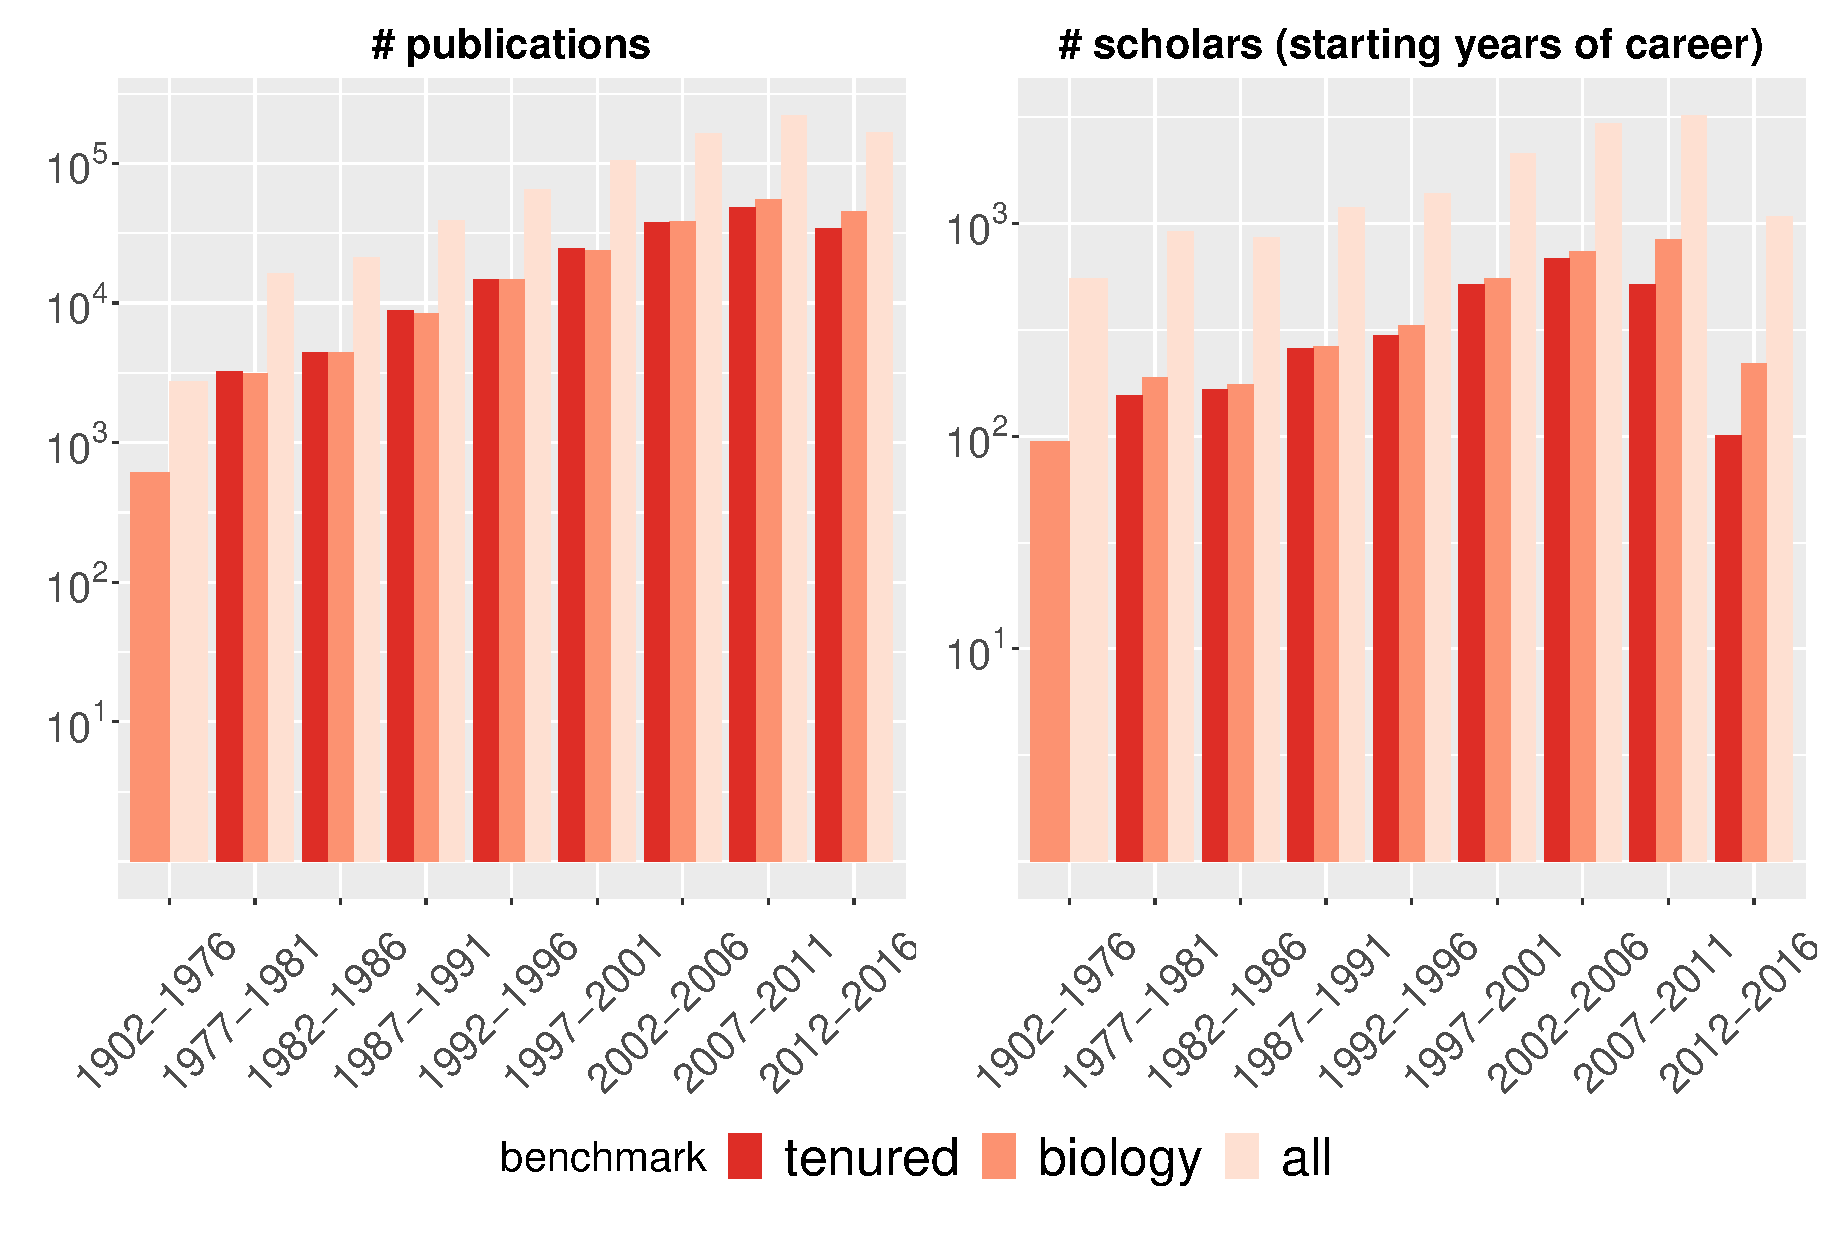
\includegraphics[width=0.8\textwidth]{figures/exploratory/npub_naut.eps}
    \caption[Exploratory statistics of the dataset]{\textbf{Left panel}: number of papers published in a certain period; \textbf{right panel}: number of authors who start their careers in a certain period. }
    \label{fig:exploratory}
\end{figure}

\begin{figure}[ht!]
    \centering
    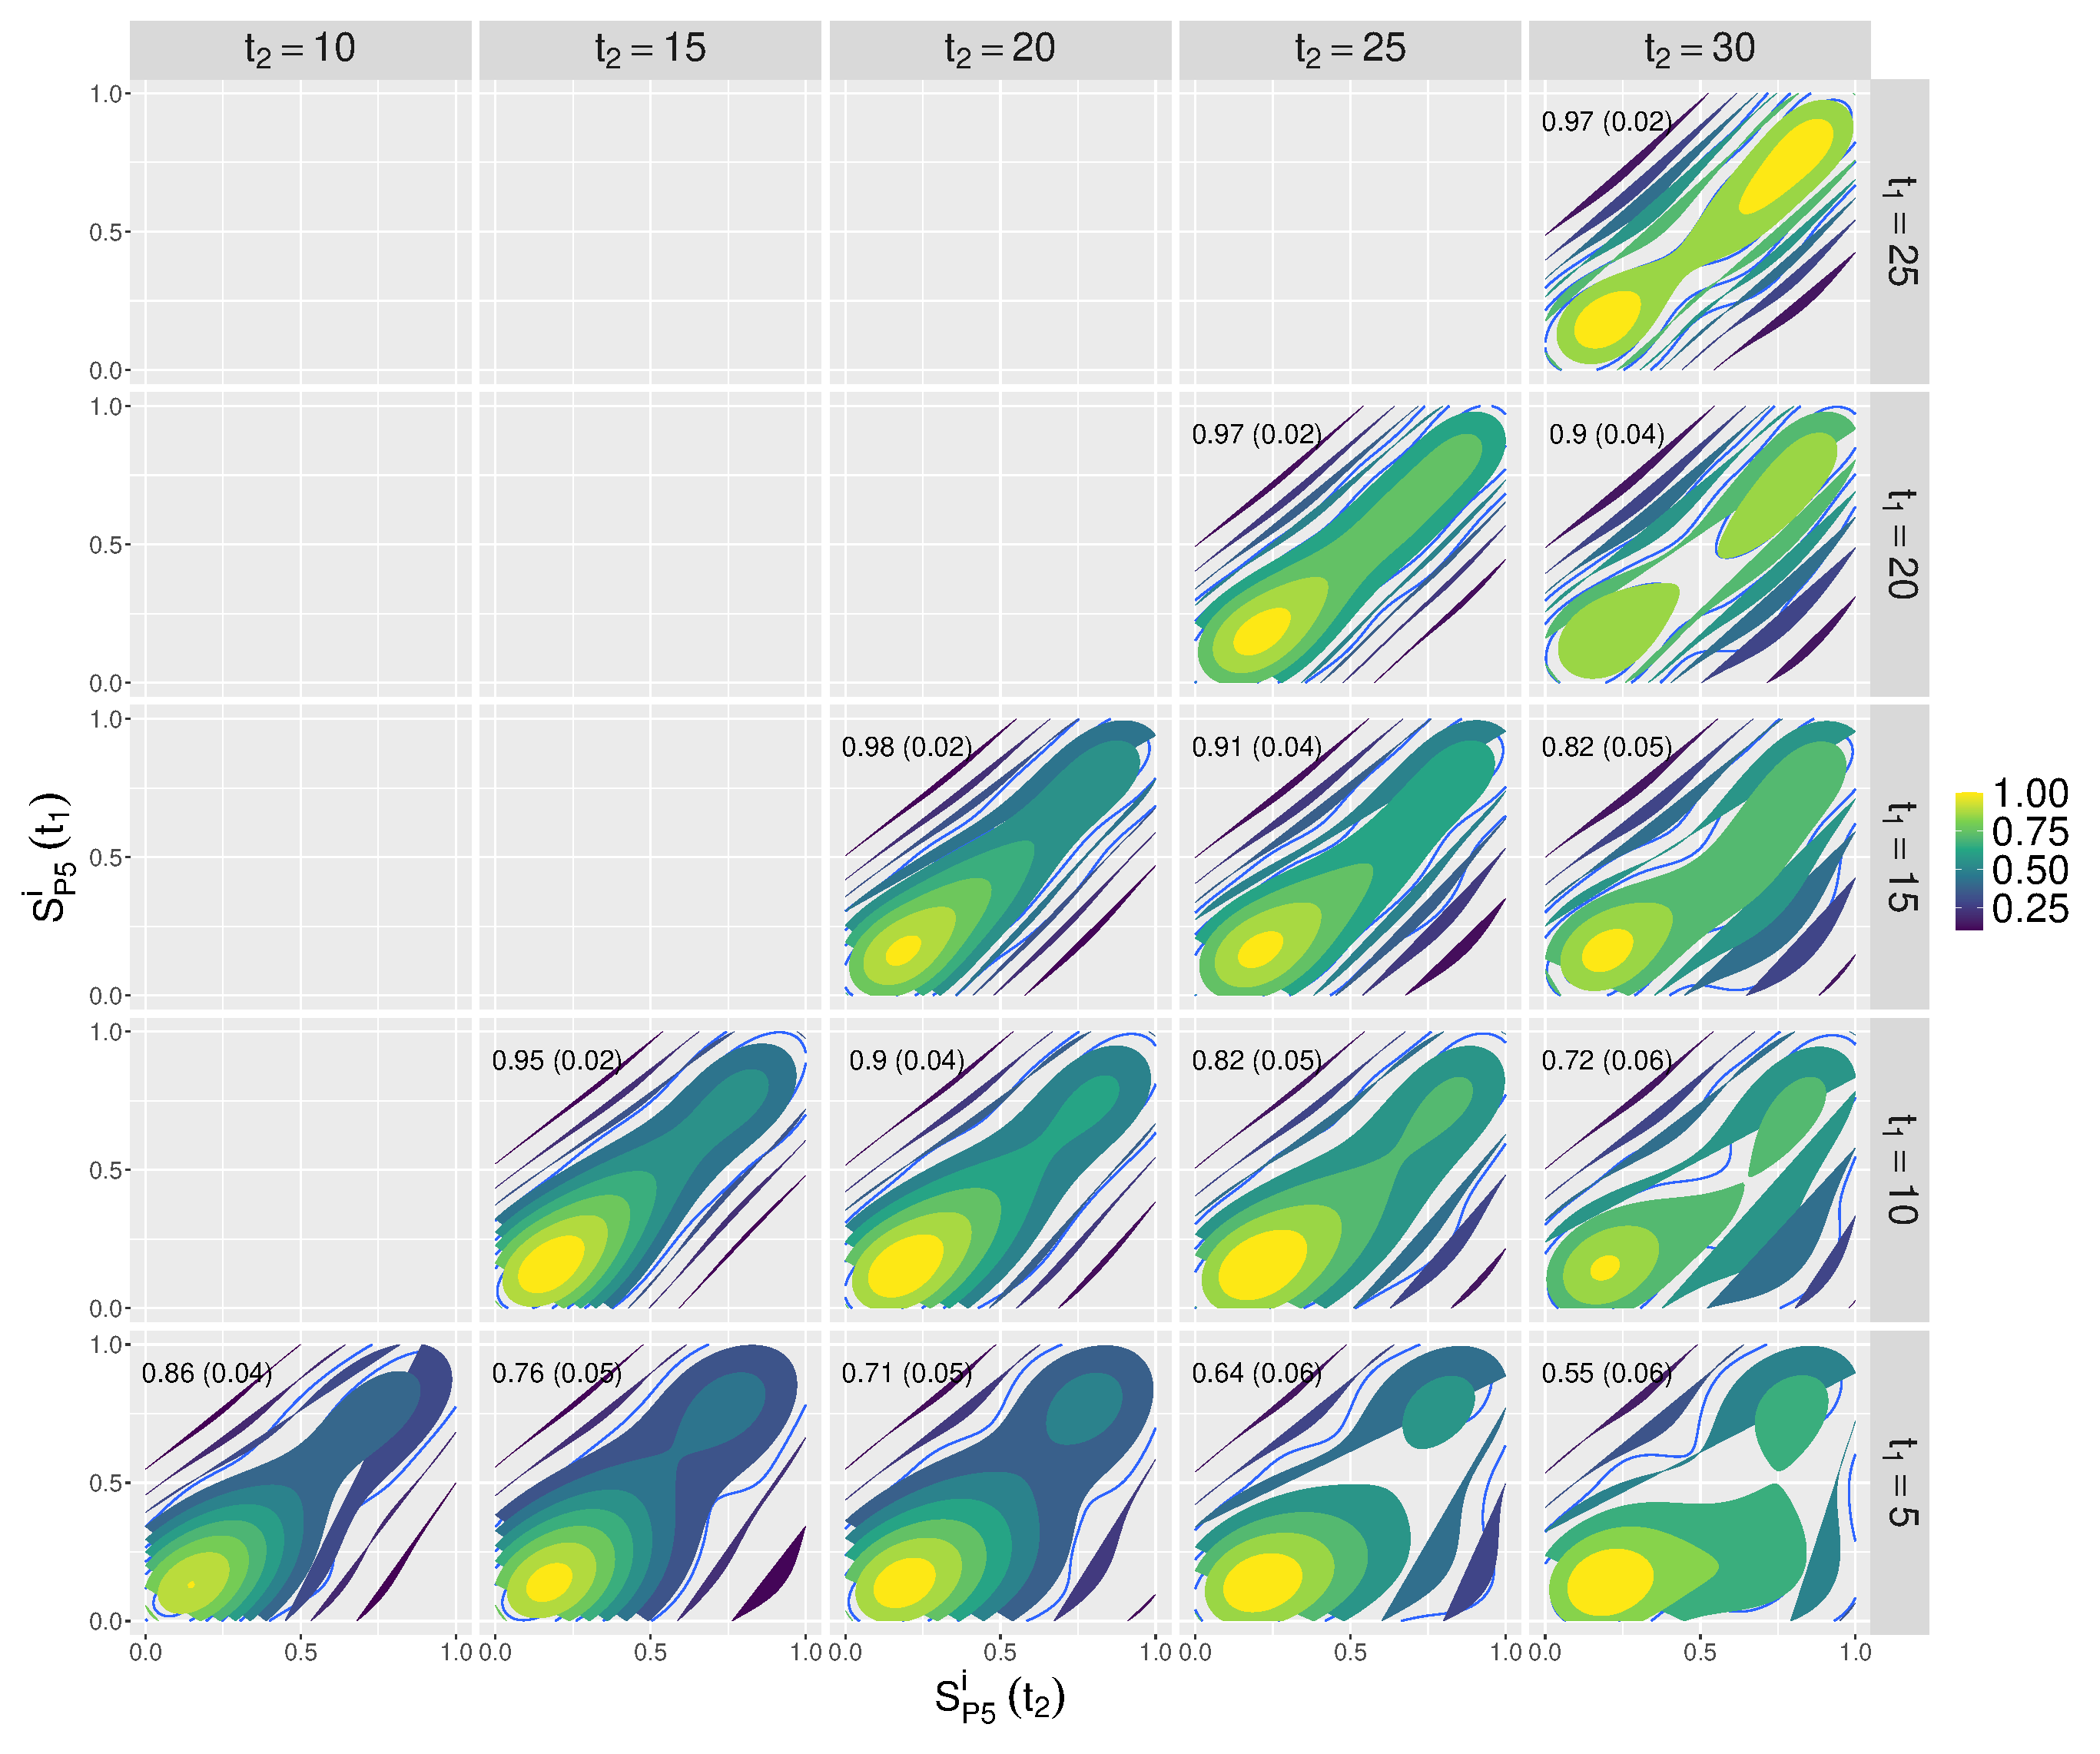
\includegraphics[width=\textwidth]{figures/pred_power/scatter_autrp_all.eps}
    \caption[Kernel density estimation for the scatters of S$_{P5}(t_1)$ and S$_{P5}(t_2)$]{Kernel density estimation for the scatter points of S$_{P5}^{ib}(t_1)$ and S$_{P5}^{ib}(t_2)$. We also fit a simple linear regression of S$_{P5}^{ib}(t_2)$ on S$_{P5}^{ib}(t_1)$. The estimated coefficient and the corresponding standard error (in the parentheses) are displayed in each plot.}
    \label{fig:scatter_autrp_all}
\end{figure}


\begin{figure}[ht!]
    \centering
    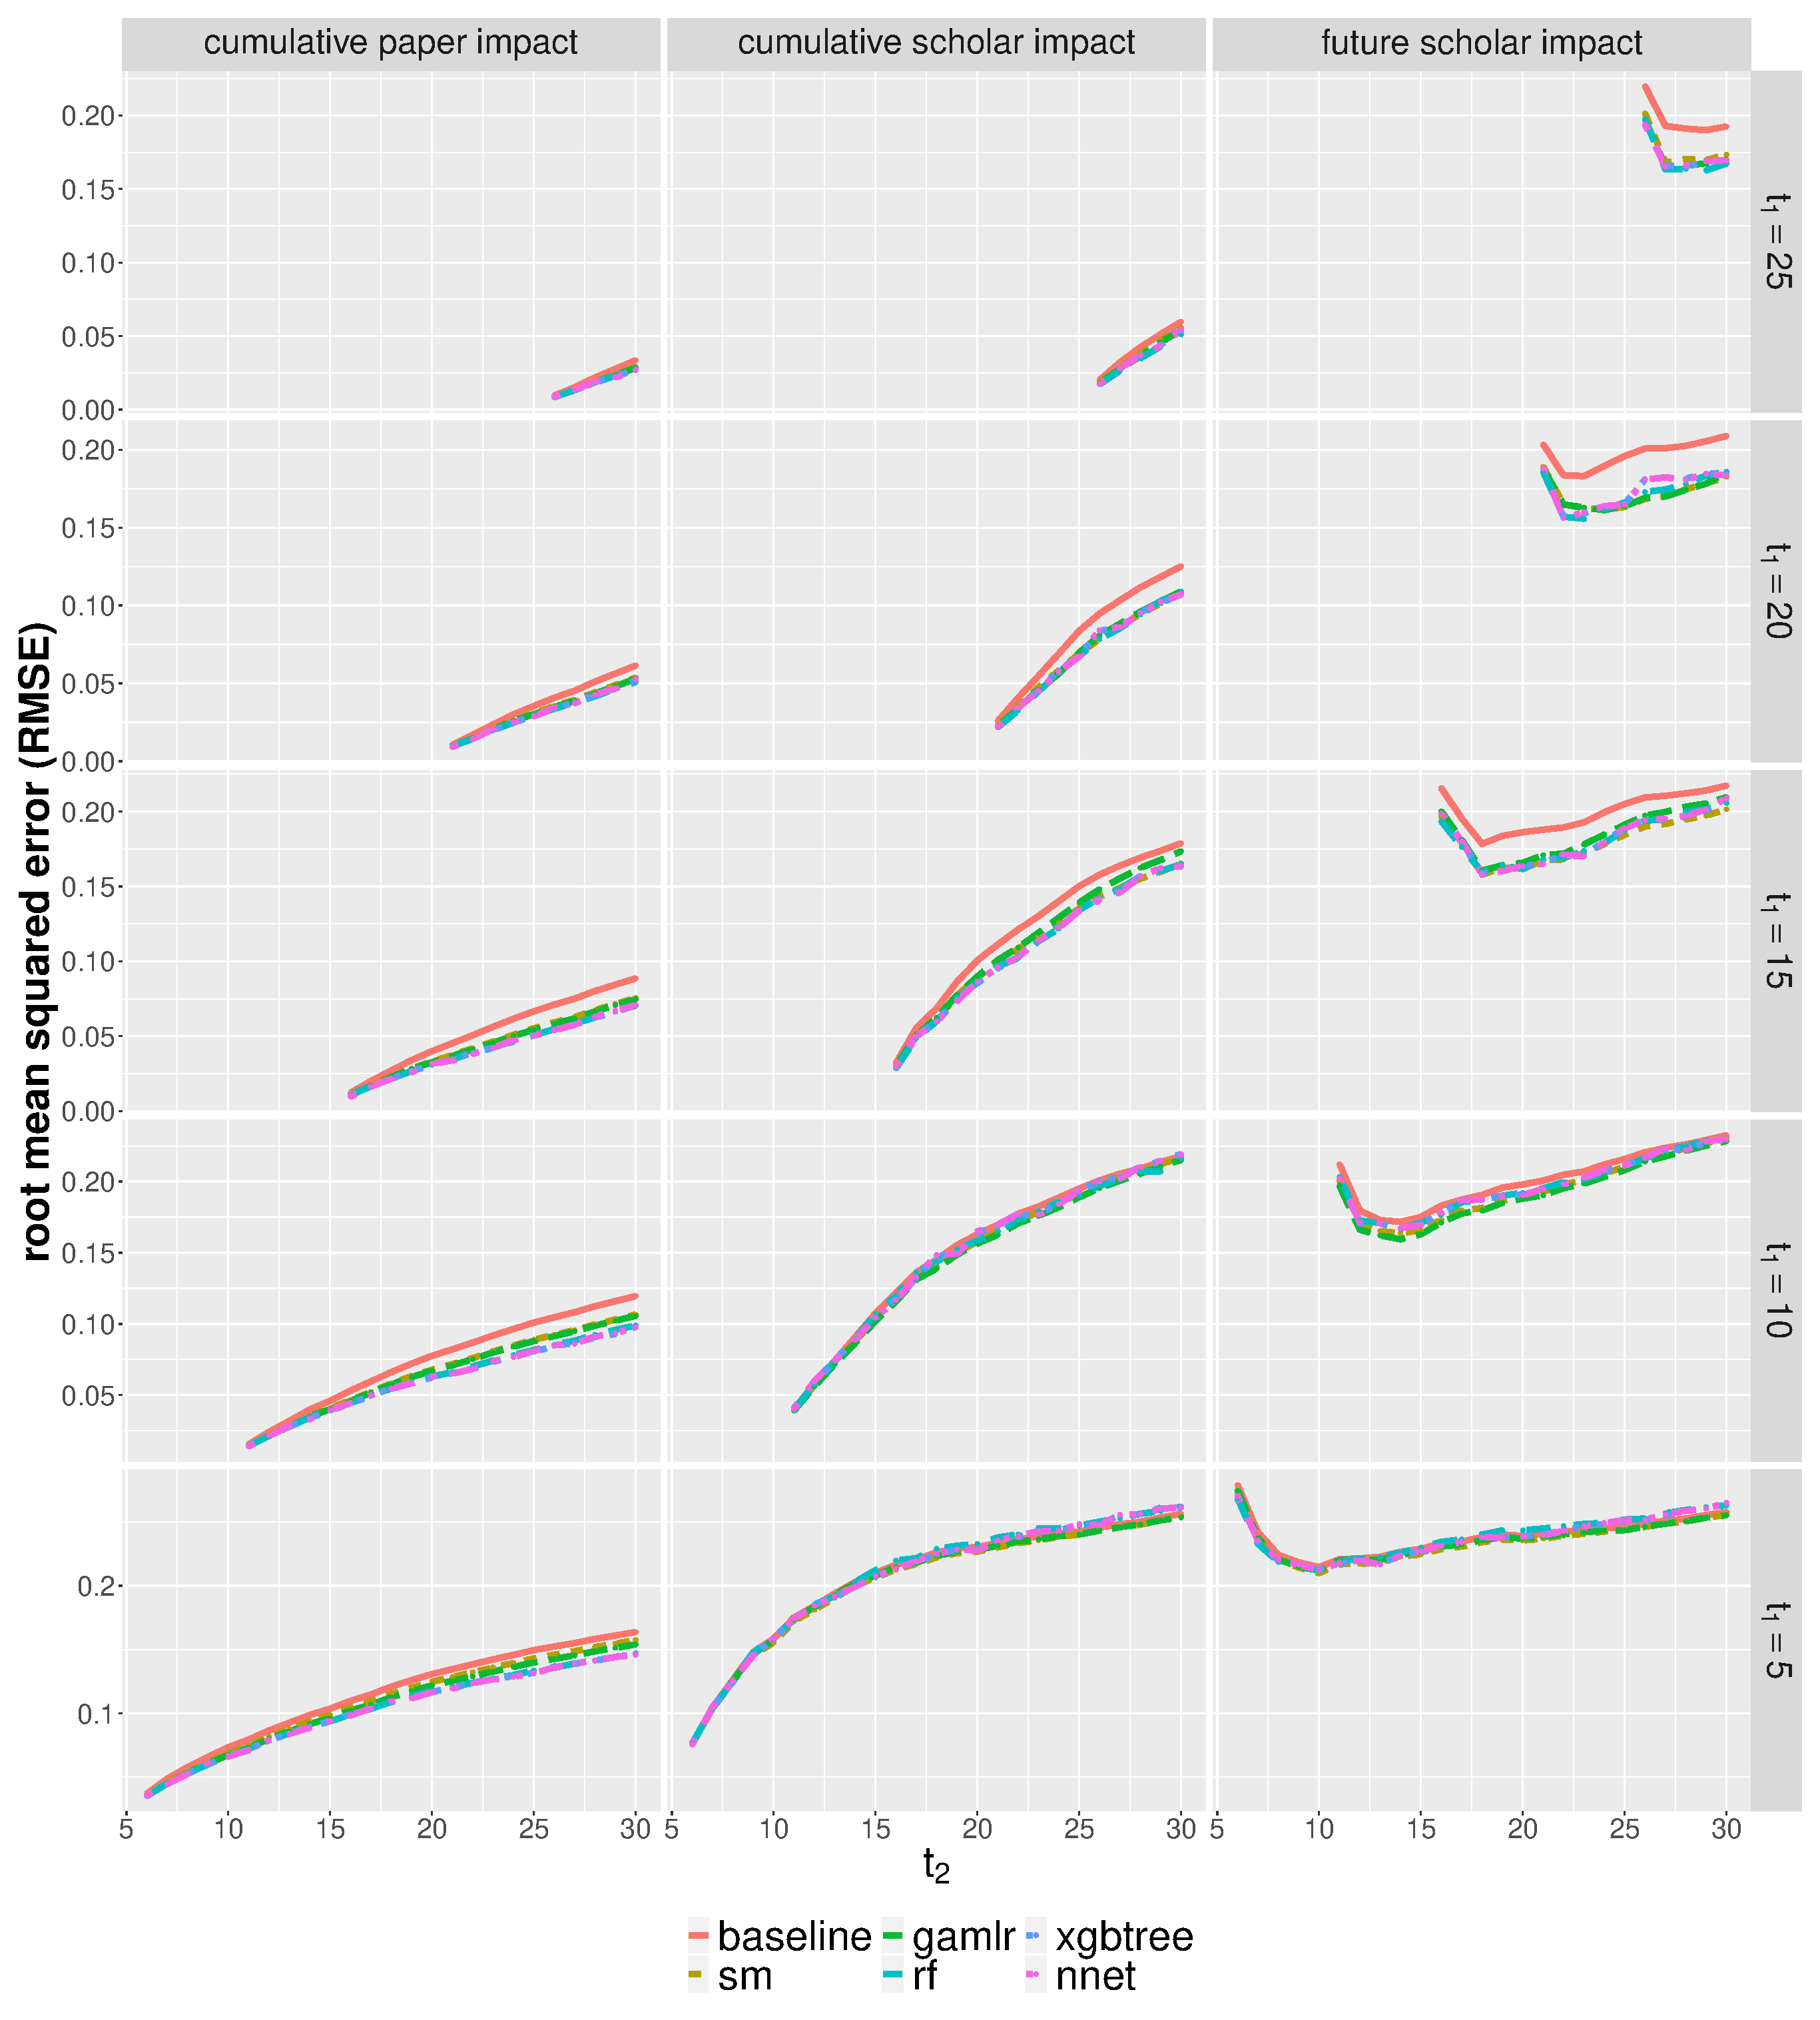
\includegraphics[width=\textwidth]{figures/pred_model/rmse.eps}
    \caption[RMSE of the predictive models]{Root mean squared error of the predictive models. The lasso, ridge and elastic net are outperformed by Gamma lasso, and hence are ignored for a better visualization.}
    \label{fig:pred_rmse}
\end{figure}

\begin{figure}[ht!]
    \centering
    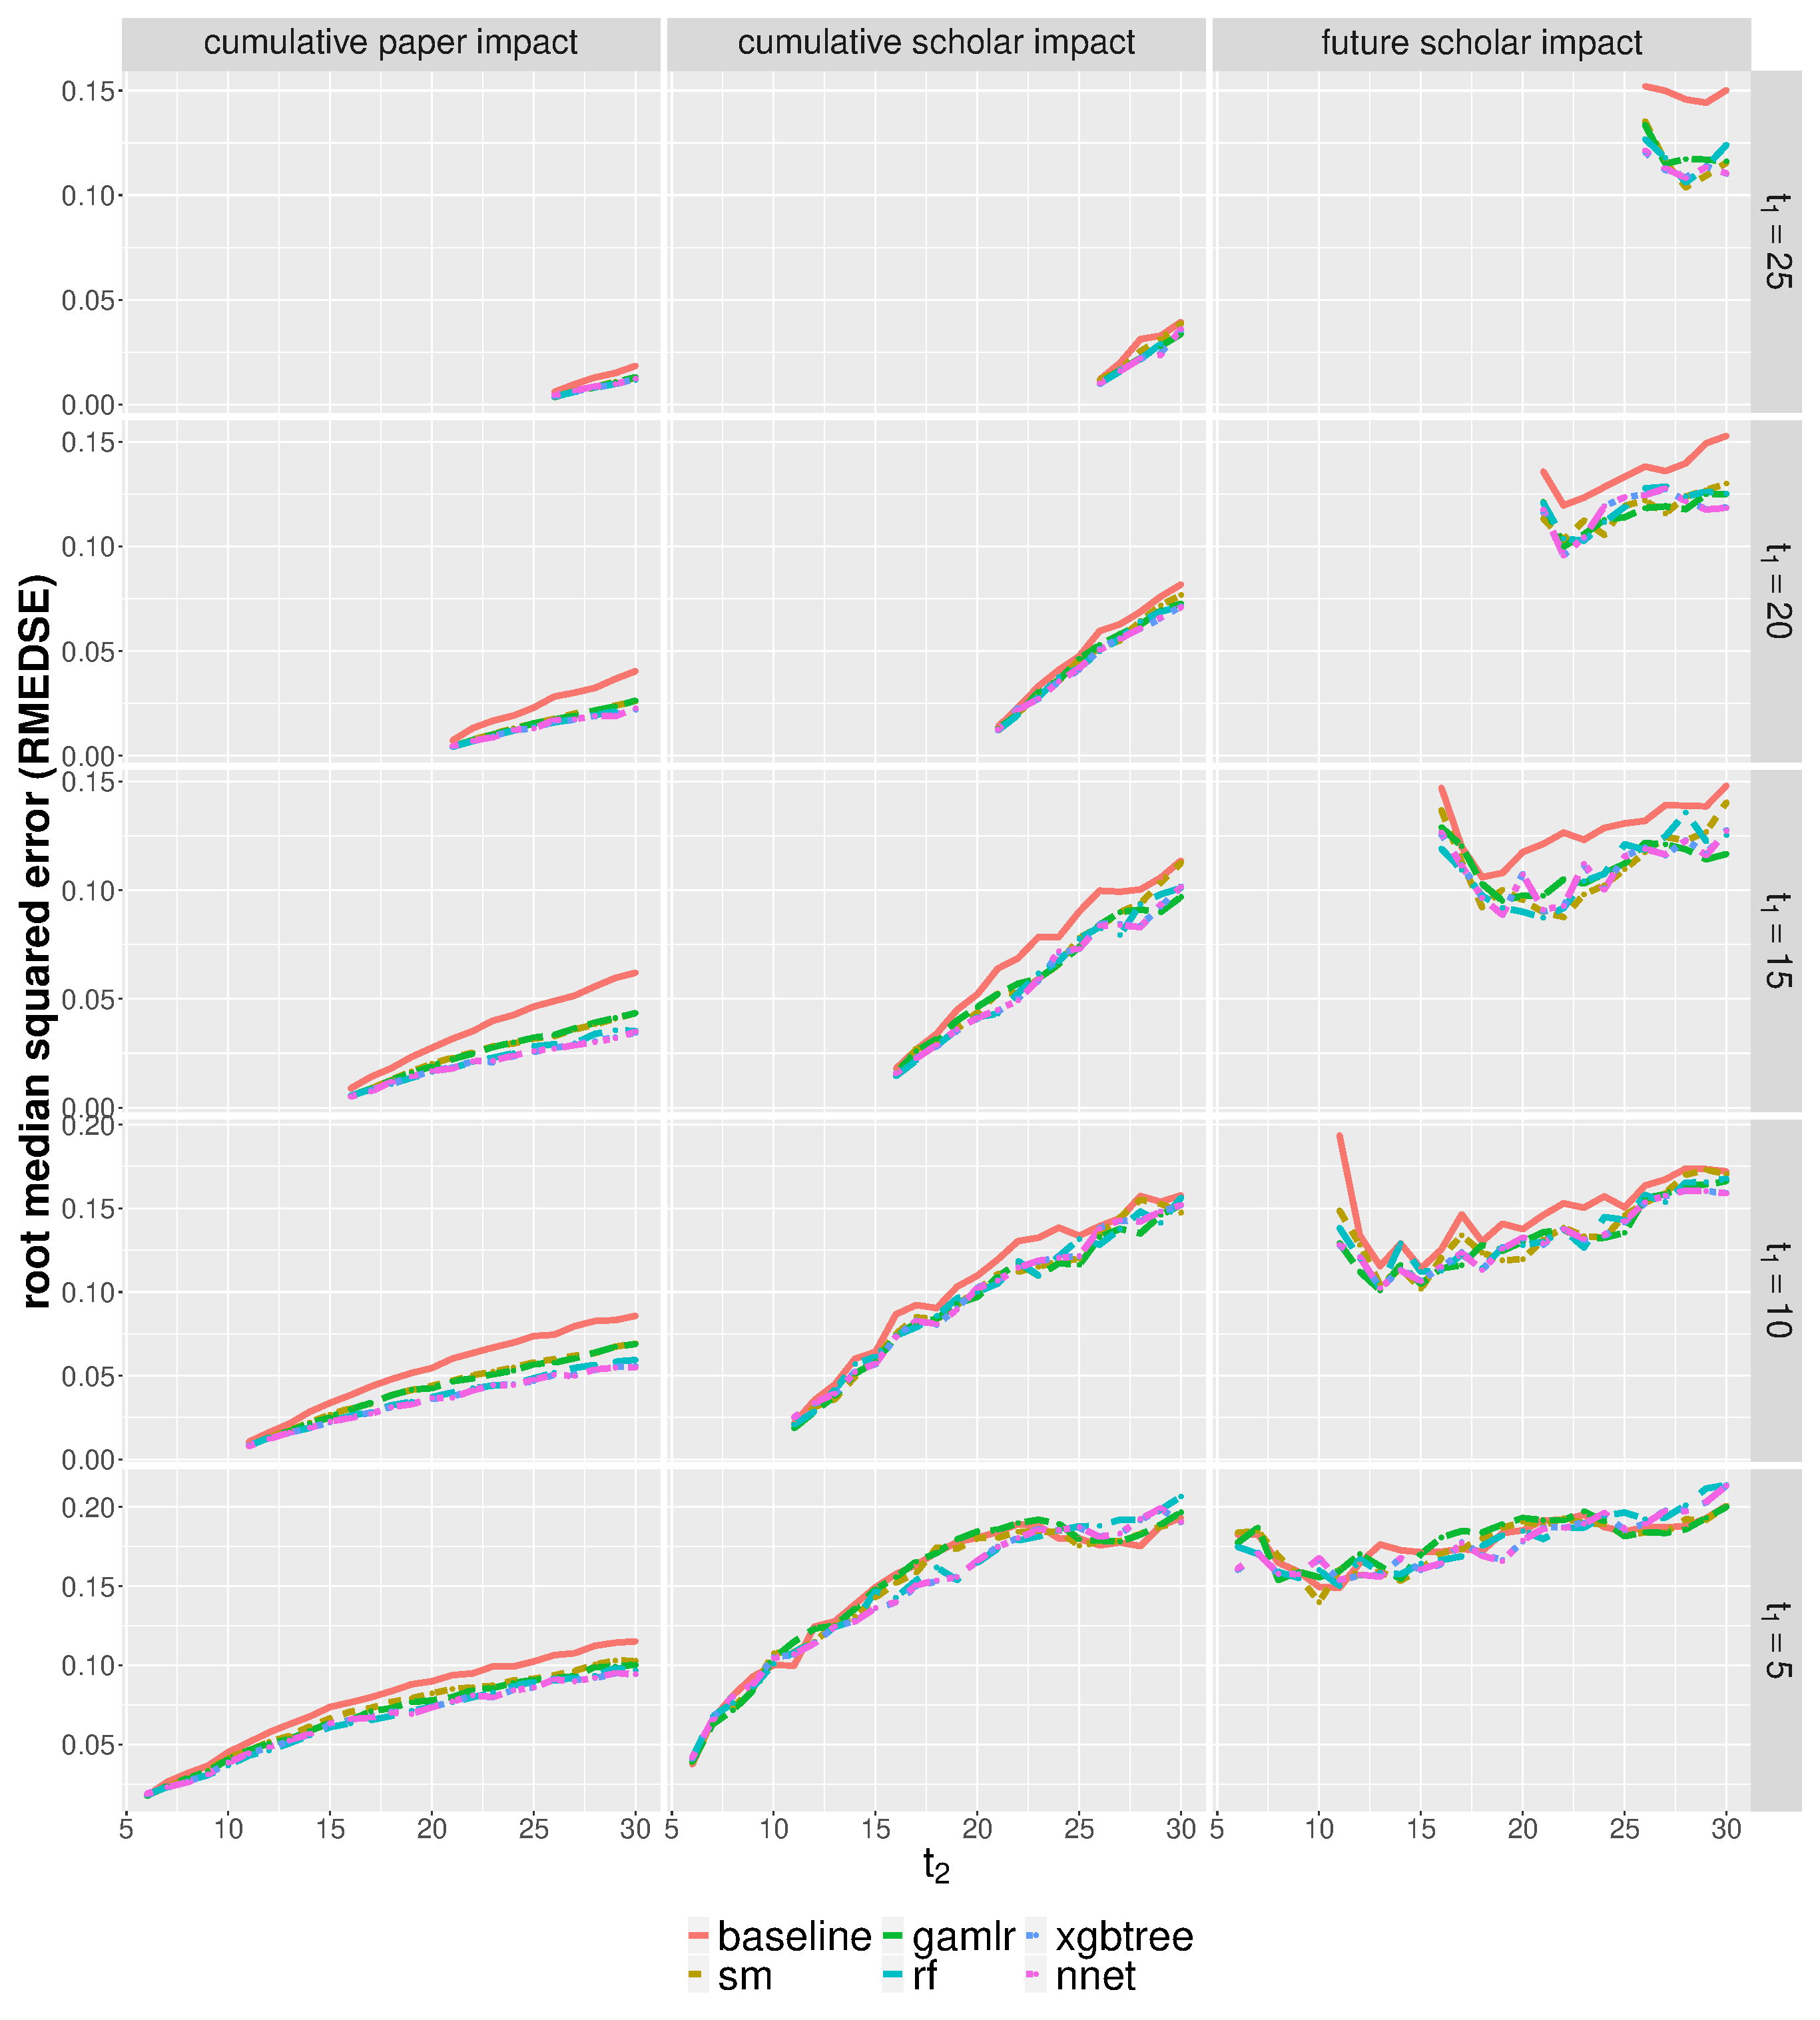
\includegraphics[width=\textwidth]{figures/pred_model/medse.eps}
    \caption[RMESE of the predictive models]{Root median squared error of the predictive models.}
    \label{fig:pred_medse}
\end{figure}

\begin{figure}[ht!]
    \centering
    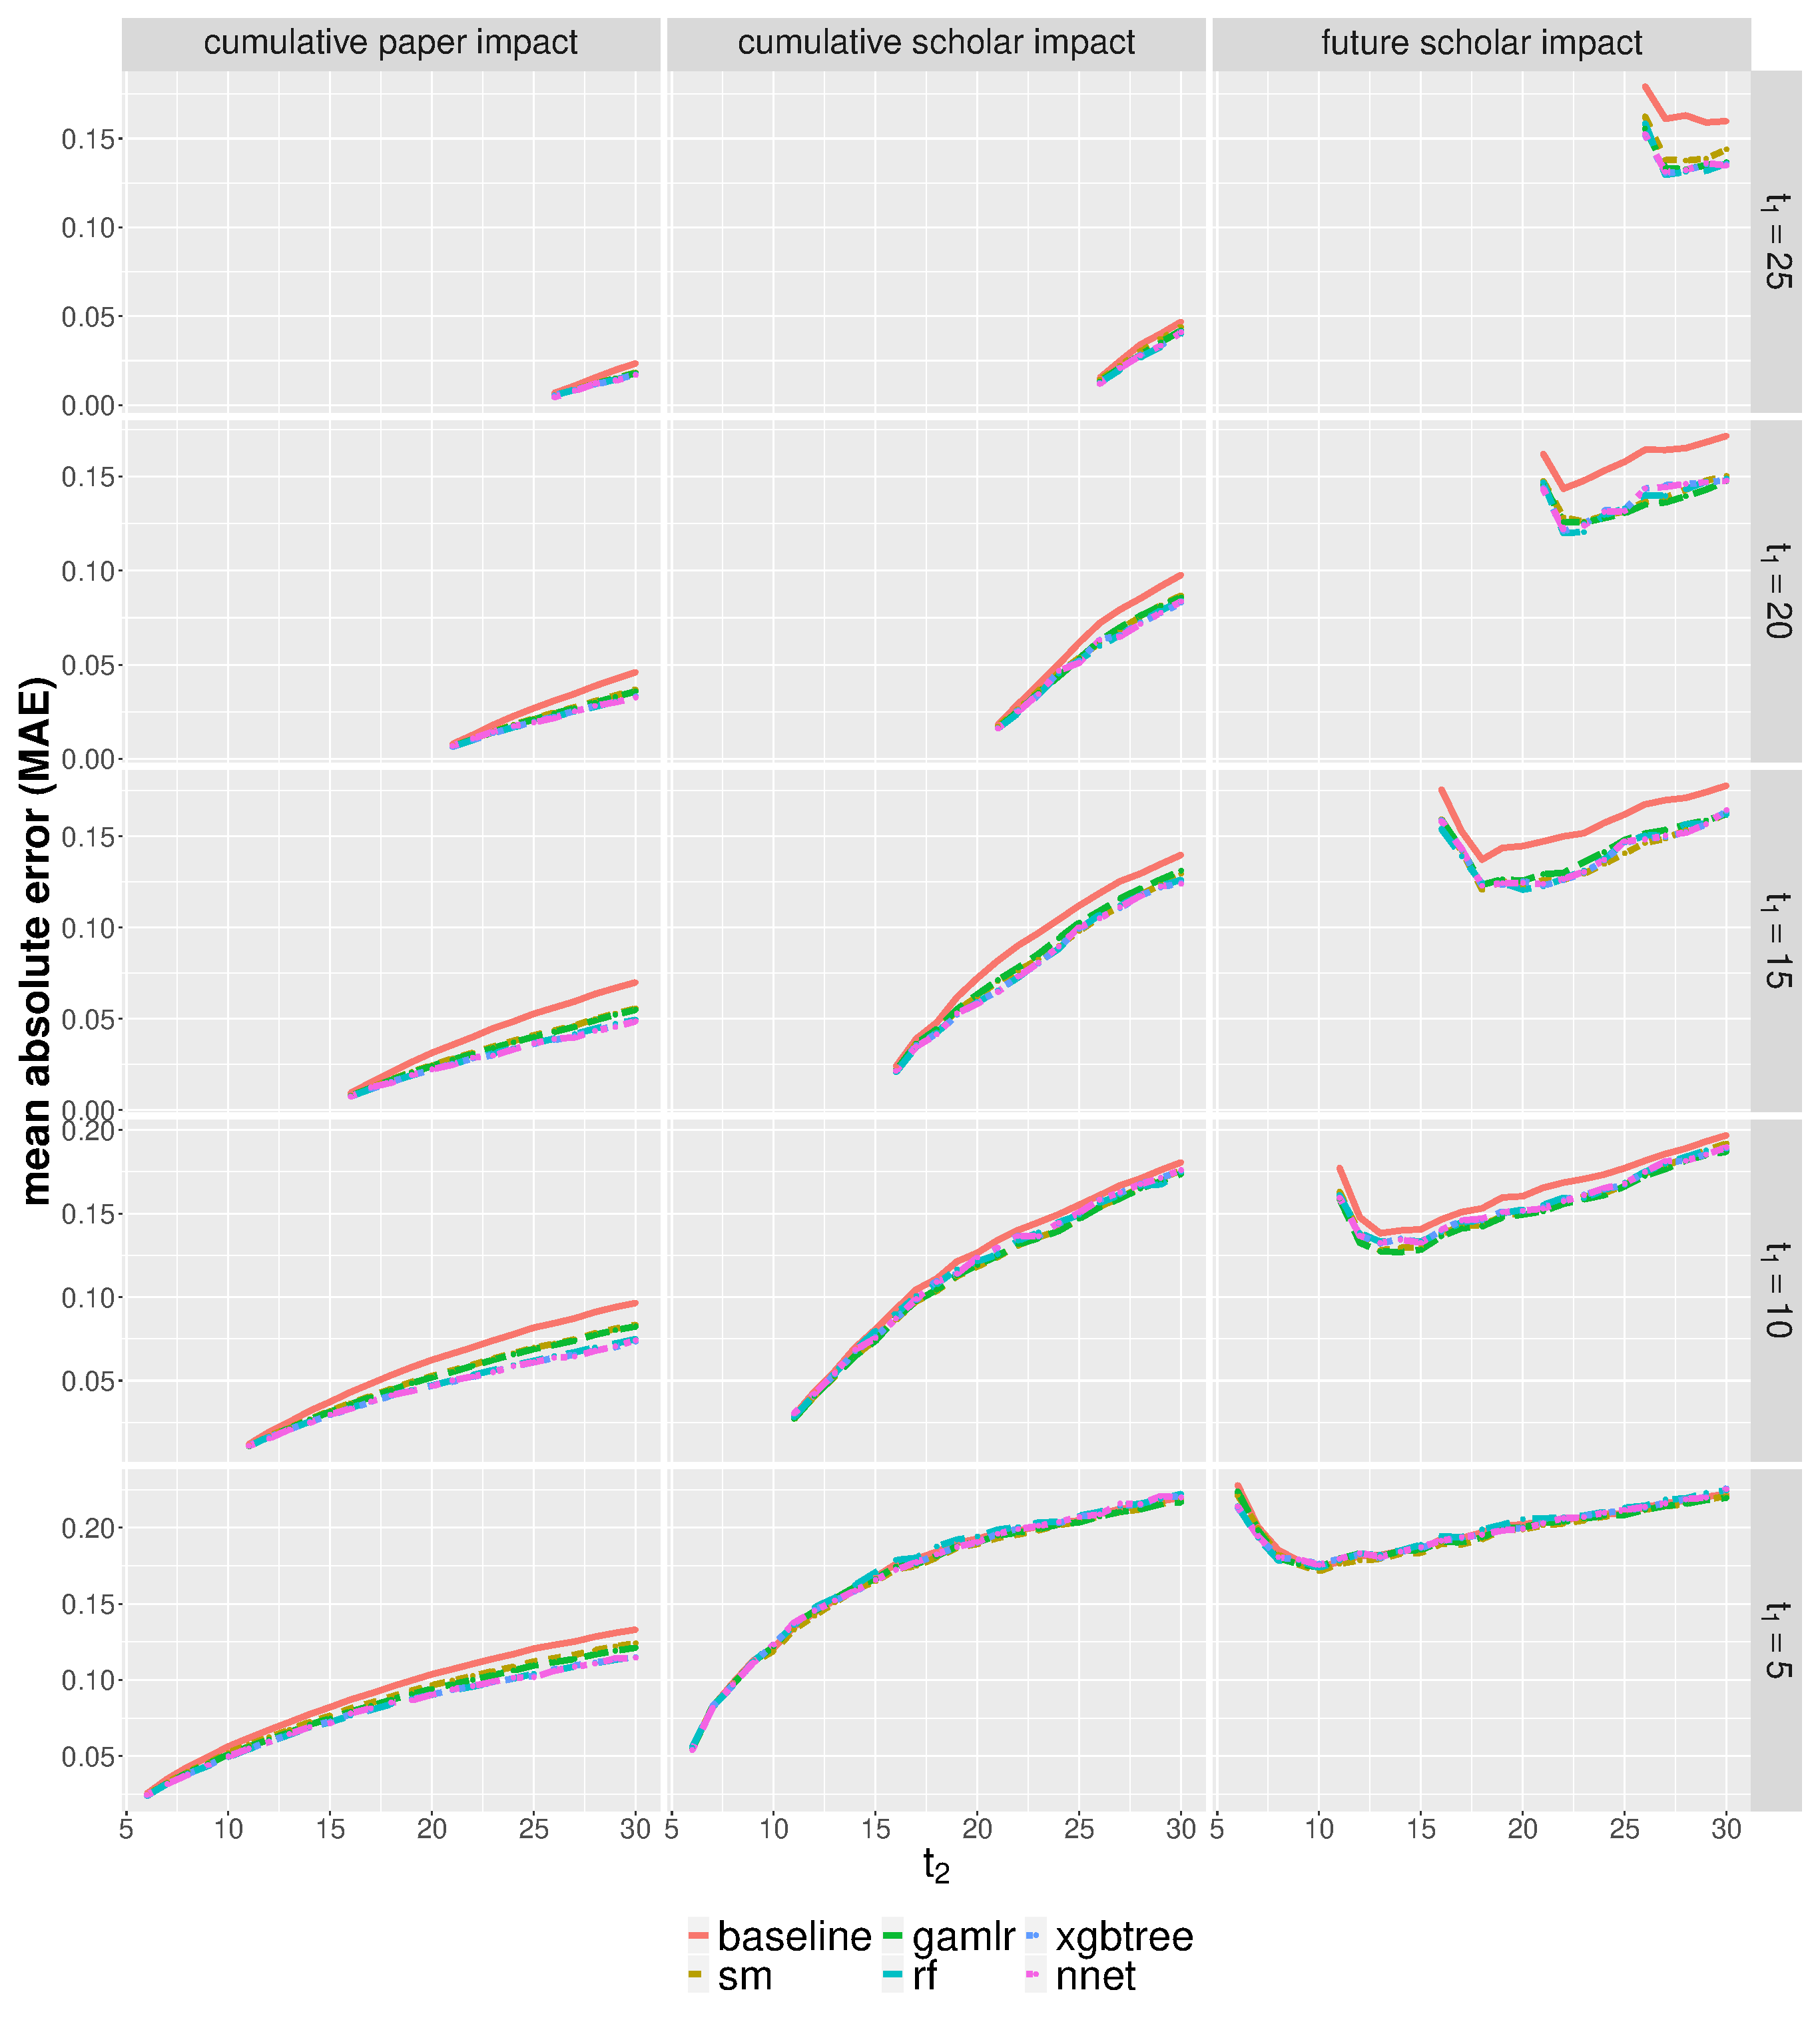
\includegraphics[width=\textwidth]{figures/pred_model/mae.eps}
    \caption[MAE of the predictive models]{Mean absolute error of the predictive models.}
    \label{fig:pred_mae}
\end{figure}

\iffalse
\clearpage
Three effects may lead to the non-stationarity of rank percentile for scholars are:
\begin{itemize}
  \item Seniority effect of scholars: senior scholars can attract more citations than junior scholars. In figure \ref{fig:seniority}, we see that senior authors (e.g. those starting their careers in 1980s) do not have an advantage over junior authors (e.g. those starting their careers in 2000s). 
  \item Time effect: papers published more recently attract more citations than papers published $20$ years ago. This maybe due to the fact that the entire scientific community is growing, and we have much more scholars now than $20$ years ago, which makes the paper visible to a larger audience and potentially attracts more citations. Meanwhile, as Internet and especially social media becomes vital, papers now have much better visibility than those $20$ years ago. Figure \ref{fig:environment} shows that for the scholars starting their careers in $1980$, more recent papers attract more citations than old papers. Since we've already filtered out the seniority effect of the scholars, this is result from external effects. 
  \item Number of publications: scholars now tend to produce more publications than scholars say $20$ years ago. Evidence is shown in figure \ref{fig:npub}. 
\end{itemize}
We now fix the bias from the time effect and number of publications, in order to get stationary rank percentile indicators for scholars. Let's say we have a scholar $i$ who starts his/her career in physical year $Y_i$. For a paper $j$ that the scholar publishes in physical year $Y_j$, we calculate its rank percentile rp.c$_{j5}$ where the benchmark contains all the papers that are published in year $Y_j$. By restricting the benchmark in such way, we potentially remove the time effect. We repeat the process for all the papers of scholar $i$ that are published by age $t$ and obtain the metric $\sum_{j=1}^{N_t^{(i)}} \text{rp.c}_{j5}$. Furthermore, we calculate a rank percentile indicator rp.p$_{it}$ based on the number of publications by age $t$, and the benchmark is all the scholars who start their careers in physical year $Y_i$. Finally, we have the evaluation metric m$_{it} = \text{rp.p}_{it} \cdot \sum_{j=1}^{N_t^{(i)}} \text{rp.c}_{j5}$. The rank percentile indicator, denoted as rp.rp5, can be then computed based on m$_{it}$ and the benchmark is all or biology. 

Figure \ref{fig:compare_autrp} shows various types of scholar rank percentile indicators. Both rp.c and rp.h, that are based on total citations and h-index, show advantages for junior scholars due to the reasons explained above. However, rp.rp5 seems to be stationary. 


\begin{figure}[h!]
     \centering
     \begin{subfigure}[b]{0.48\textwidth}
         \centering
         
\includegraphics[width=\textwidth]{figures/exploratory/seniority_age5.eps}
         \caption{Total citations by age $5$ for papers published in $2012$}
     \end{subfigure}
     \hfill
     \begin{subfigure}[b]{0.5\textwidth}
         \centering
         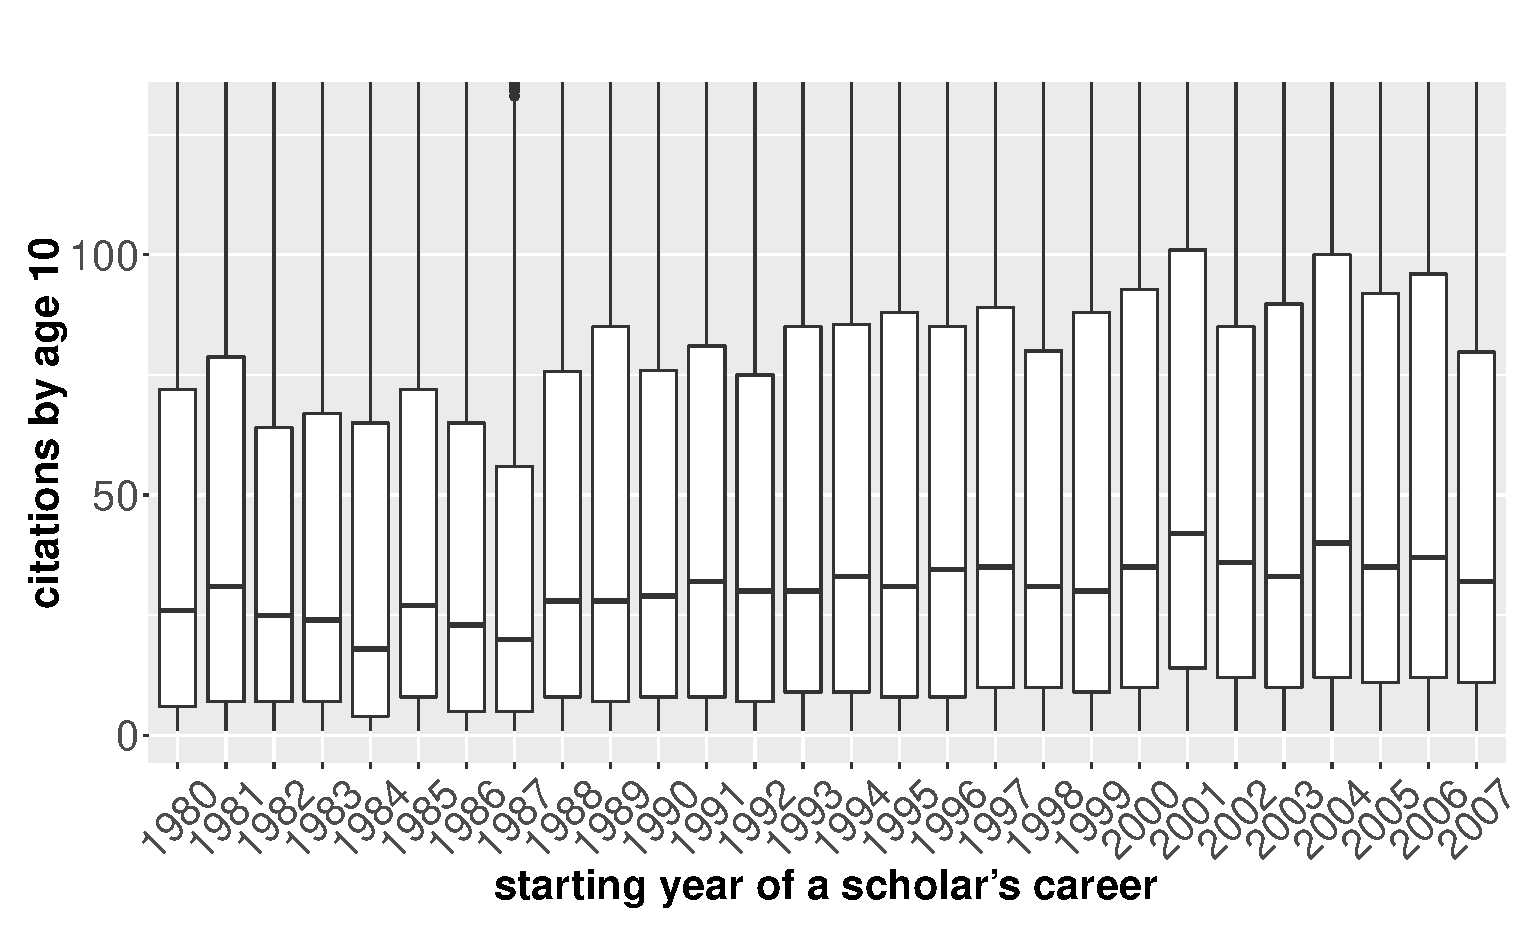
\includegraphics[width=\textwidth]{figures/exploratory/seniority_age10.eps}
         \caption{Total citations by age $10$ for papers published in $2007$}
     \end{subfigure}
    \caption{Seniority effect of scholars. The x-axis indicates starting years of careers of the corresponding authors. There's no evidence that senior scholars can attract more citations than junior scholars.}
    \label{fig:seniority}
\end{figure}

\begin{figure}[h!]
     \centering
     \begin{subfigure}[b]{0.48\textwidth}
         \centering
         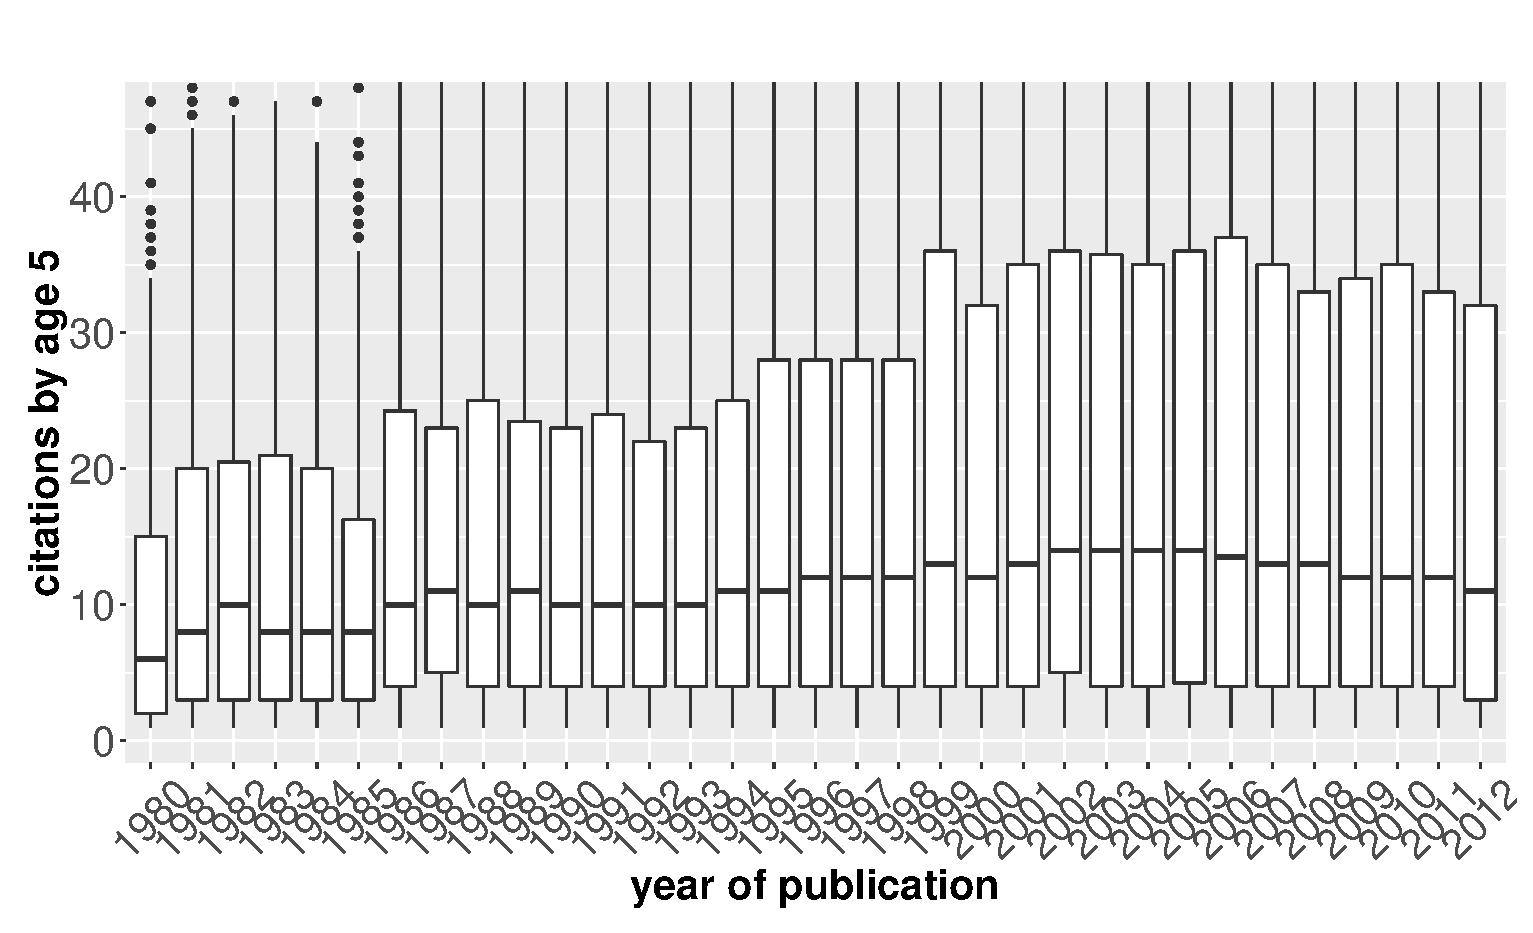
\includegraphics[width=\textwidth]{figures/exploratory/environment_age5.eps}
         \caption{Total citations by age $5$}
     \end{subfigure}
     \hfill
     \begin{subfigure}[b]{0.48\textwidth}
         \centering
         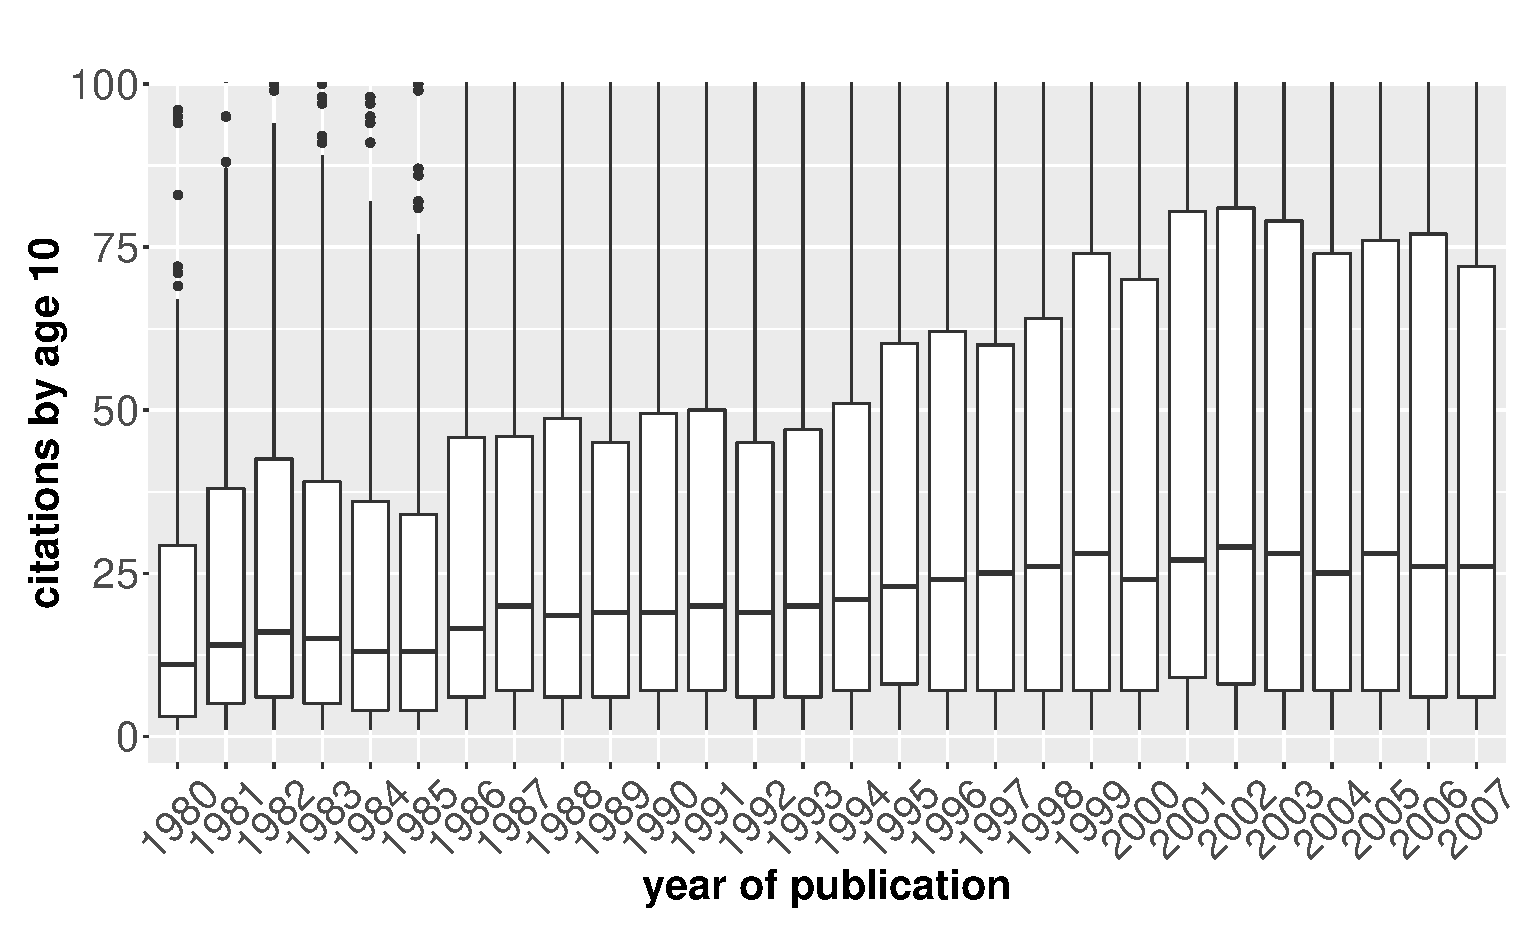
\includegraphics[width=\textwidth]{figures/exploratory/environment_age10.eps}
         \caption{Total citations by age $10$}
     \end{subfigure}
    \caption{Time effect. We consider the citations of the papers published by scholars who start their careers in year $1980$. The x-axis indicates the years of publication for their papers. We observe that more recent papers attract more citations than old papers.}
    \label{fig:environment}
\end{figure}

\begin{figure}[h!]
     \centering
     \begin{subfigure}[b]{0.48\textwidth}
         \centering
         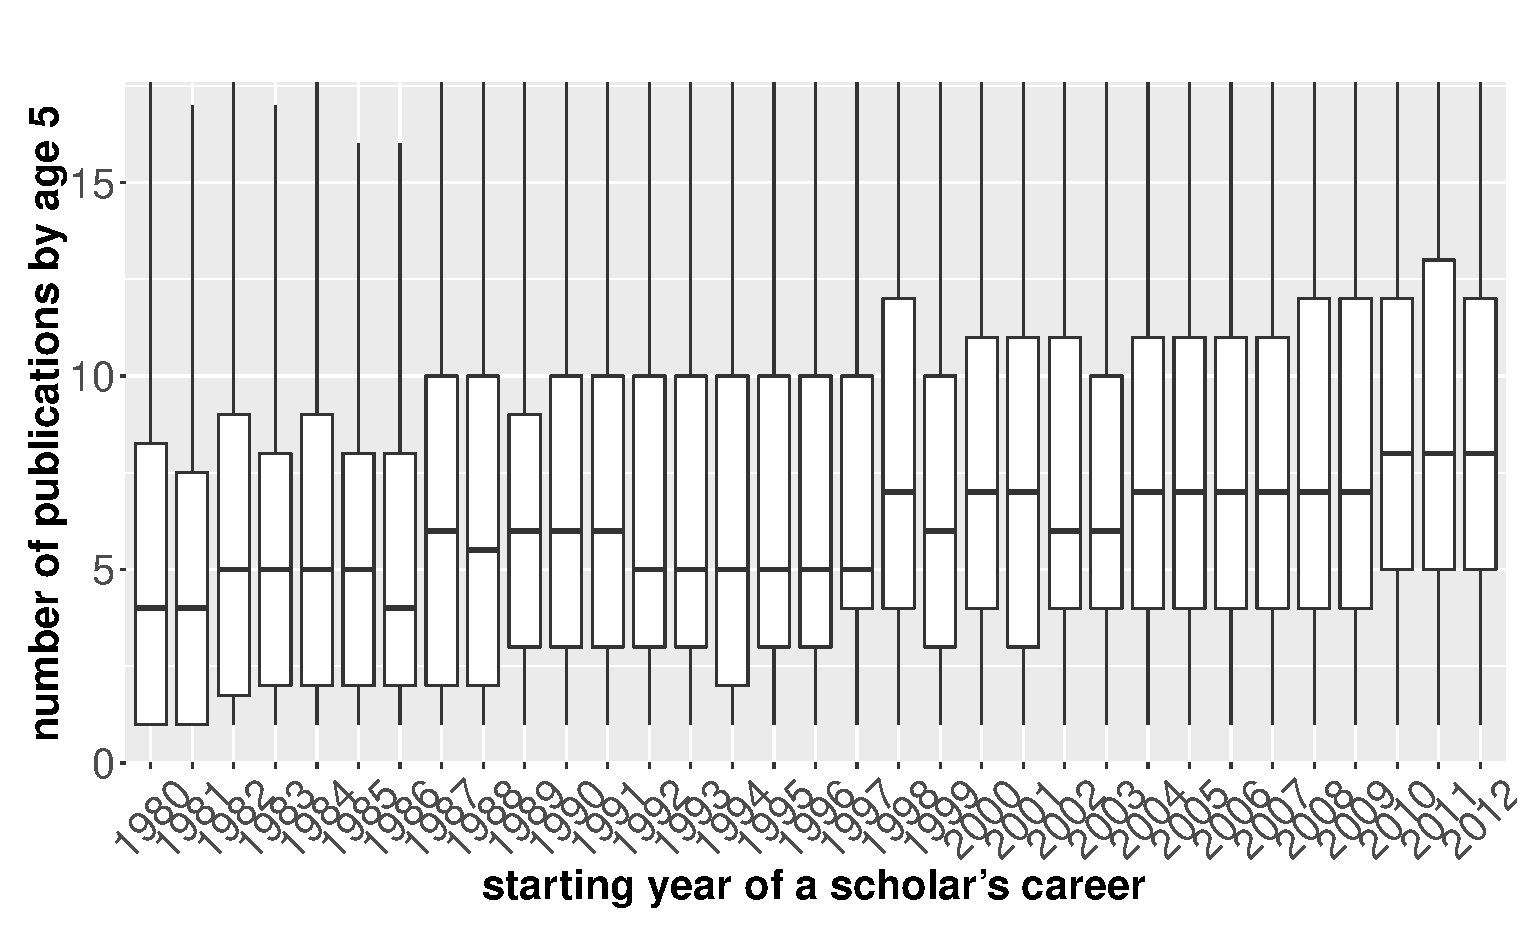
\includegraphics[width=\textwidth]{figures/exploratory/npub_age5.eps}
         \caption{Number of publications by age $5$}
     \end{subfigure}
     \hfill
     \begin{subfigure}[b]{0.48\textwidth}
         \centering
         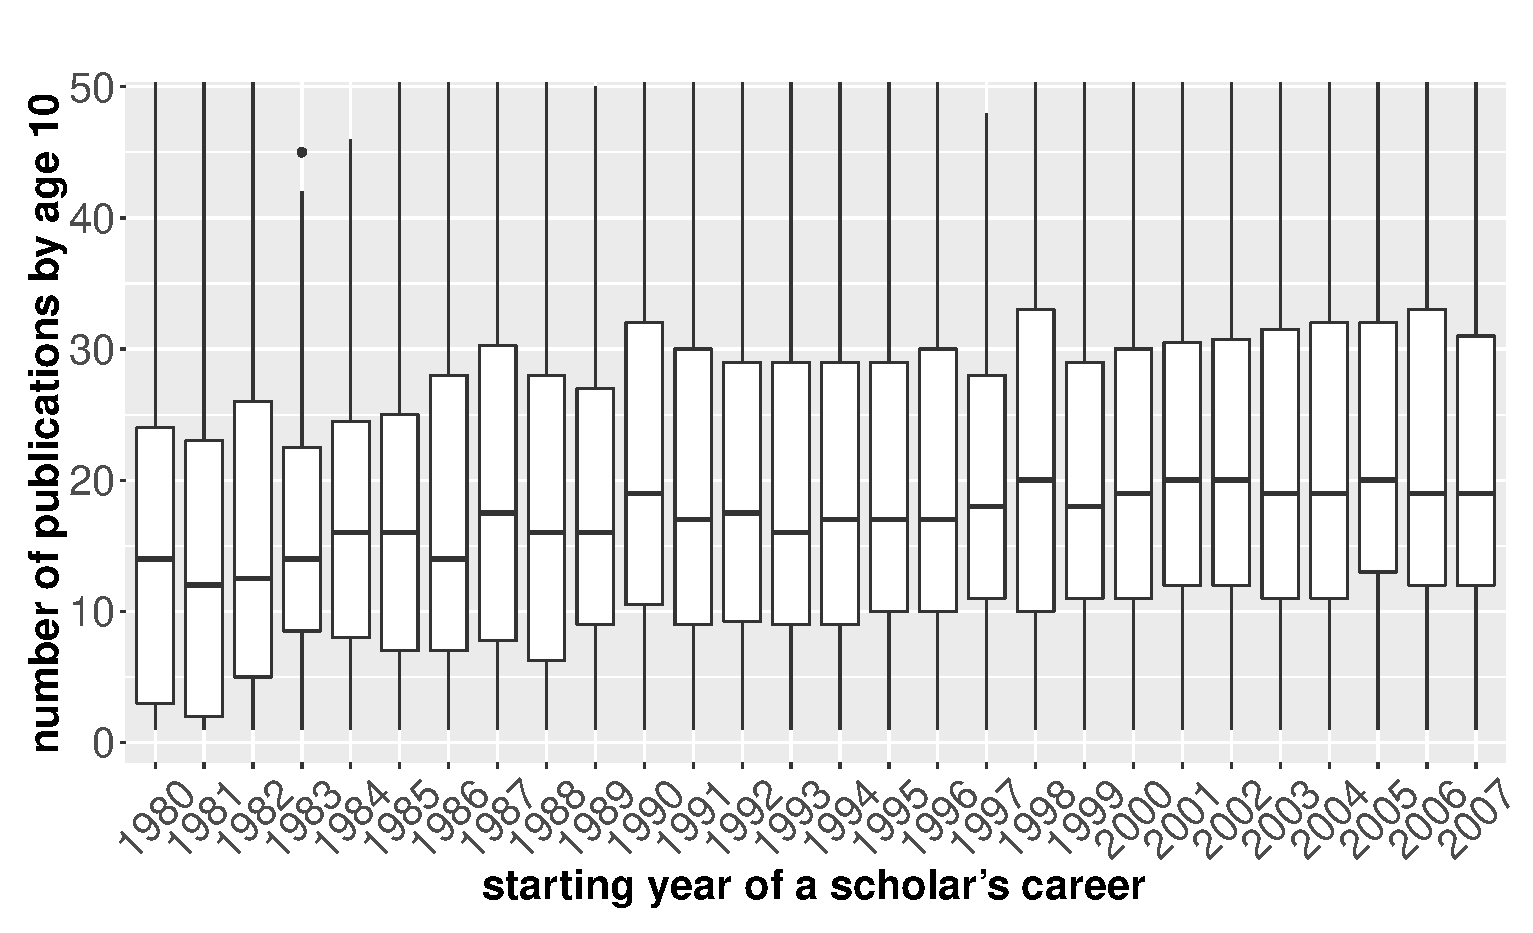
\includegraphics[width=\textwidth]{figures/exploratory/npub_age10.eps}
         \caption{Number of publications by age $10$}
     \end{subfigure}
    \caption{Number of publications. The x-axis indicates the starting years of careers of scholars. }
    \label{fig:npub}
\end{figure}


\begin{figure}[h!]
     \centering
     \begin{subfigure}[b]{0.48\textwidth}
         \centering
         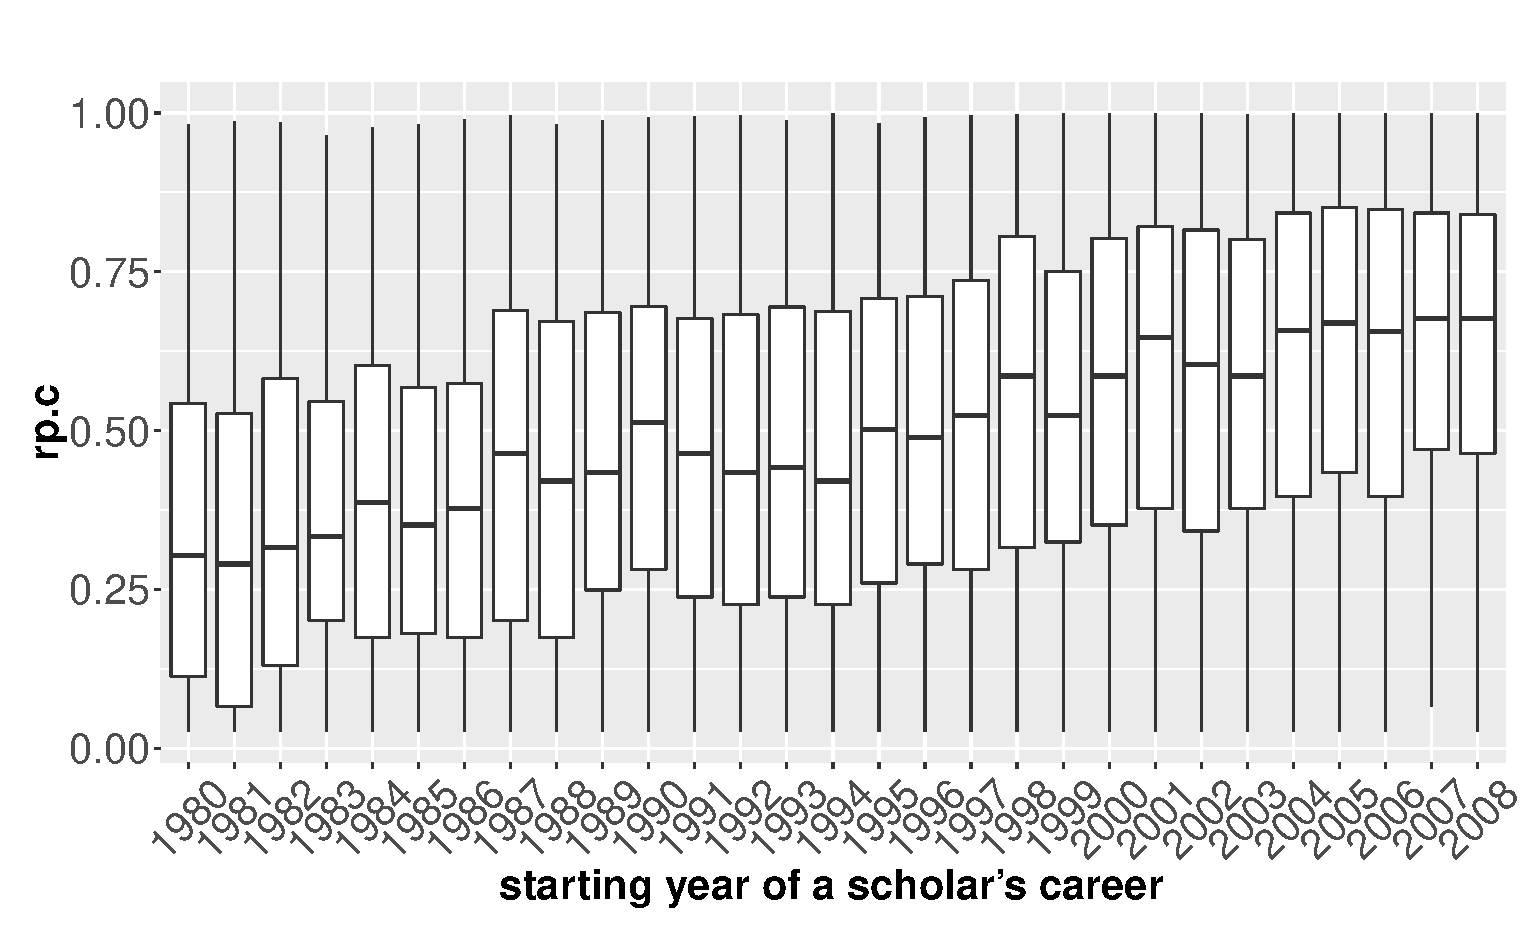
\includegraphics[width=\textwidth]{figures/exploratory/rpc_age5.eps}
         \caption{rp.c$_{i5}$}
     \end{subfigure}
     \hfill
     \begin{subfigure}[b]{0.48\textwidth}
         \centering
         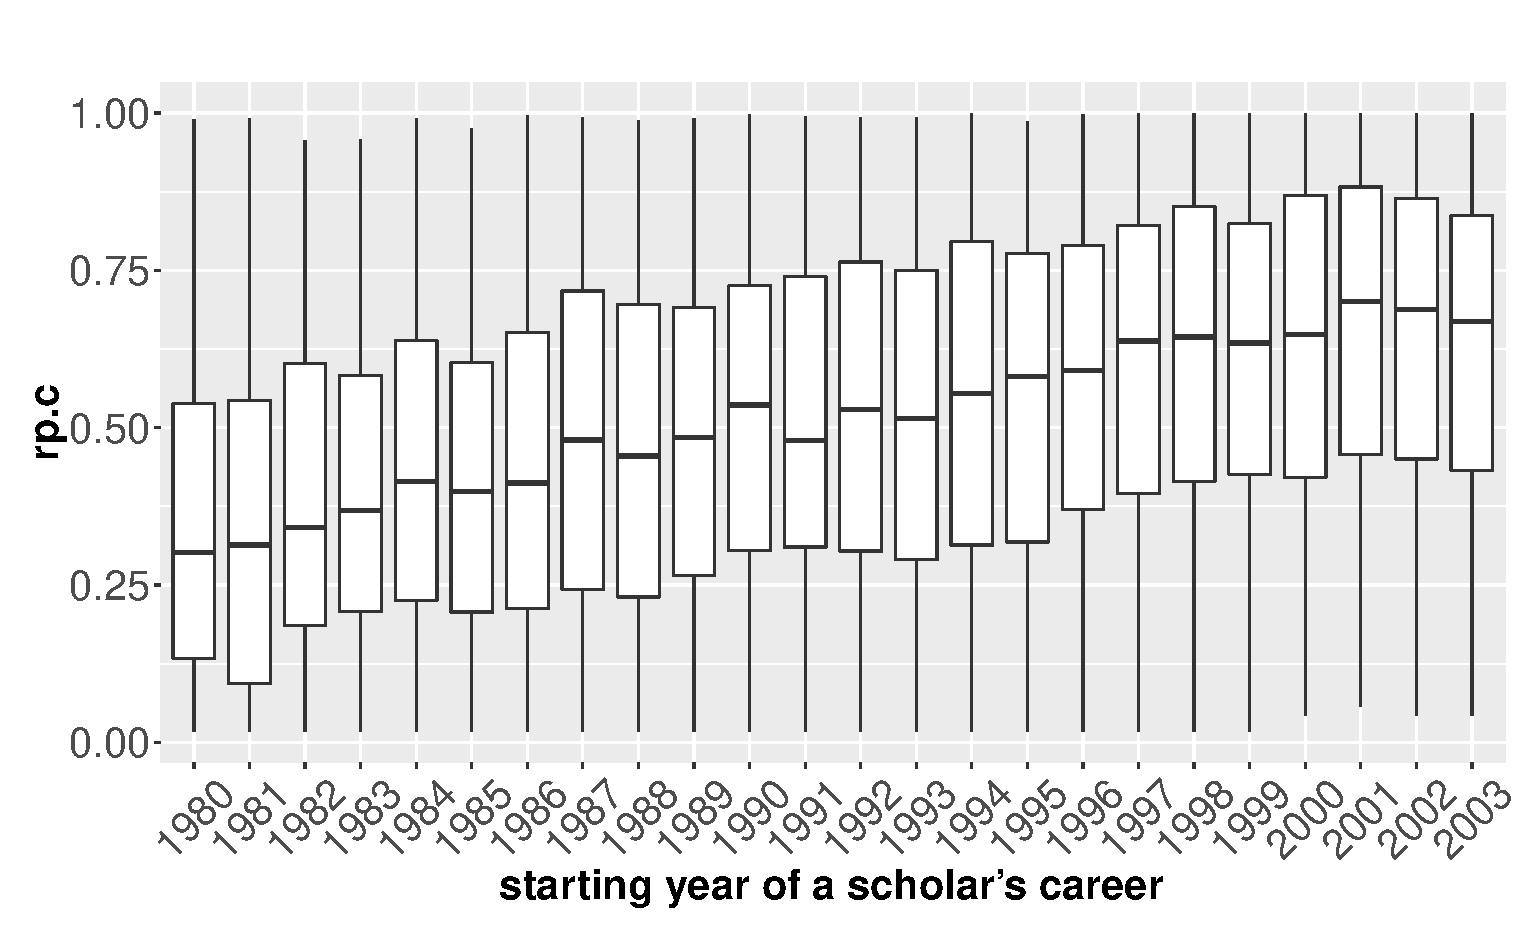
\includegraphics[width=\textwidth]{figures/exploratory/rpc_age10.eps}
         \caption{rp.c$_{i10}$}
     \end{subfigure}
     \hfill
      \begin{subfigure}[b]{0.48\textwidth}
         \centering
         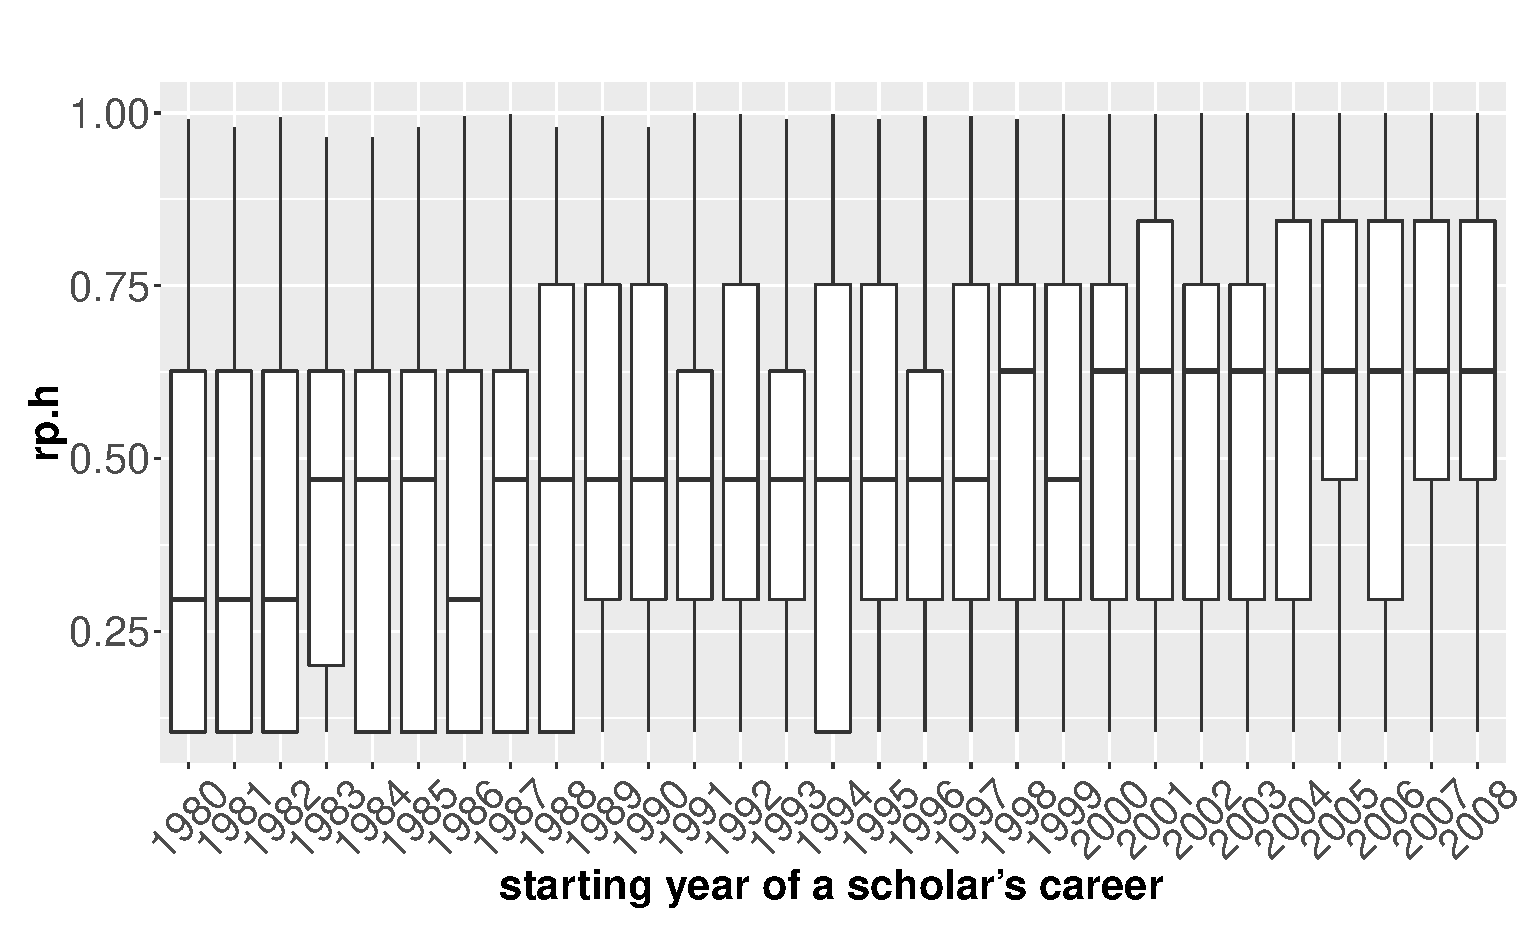
\includegraphics[width=\textwidth]{figures/exploratory/rph_age5.eps}
         \caption{rp.h$_{i5}$}
     \end{subfigure}
     \hfill
     \begin{subfigure}[b]{0.48\textwidth}
         \centering
         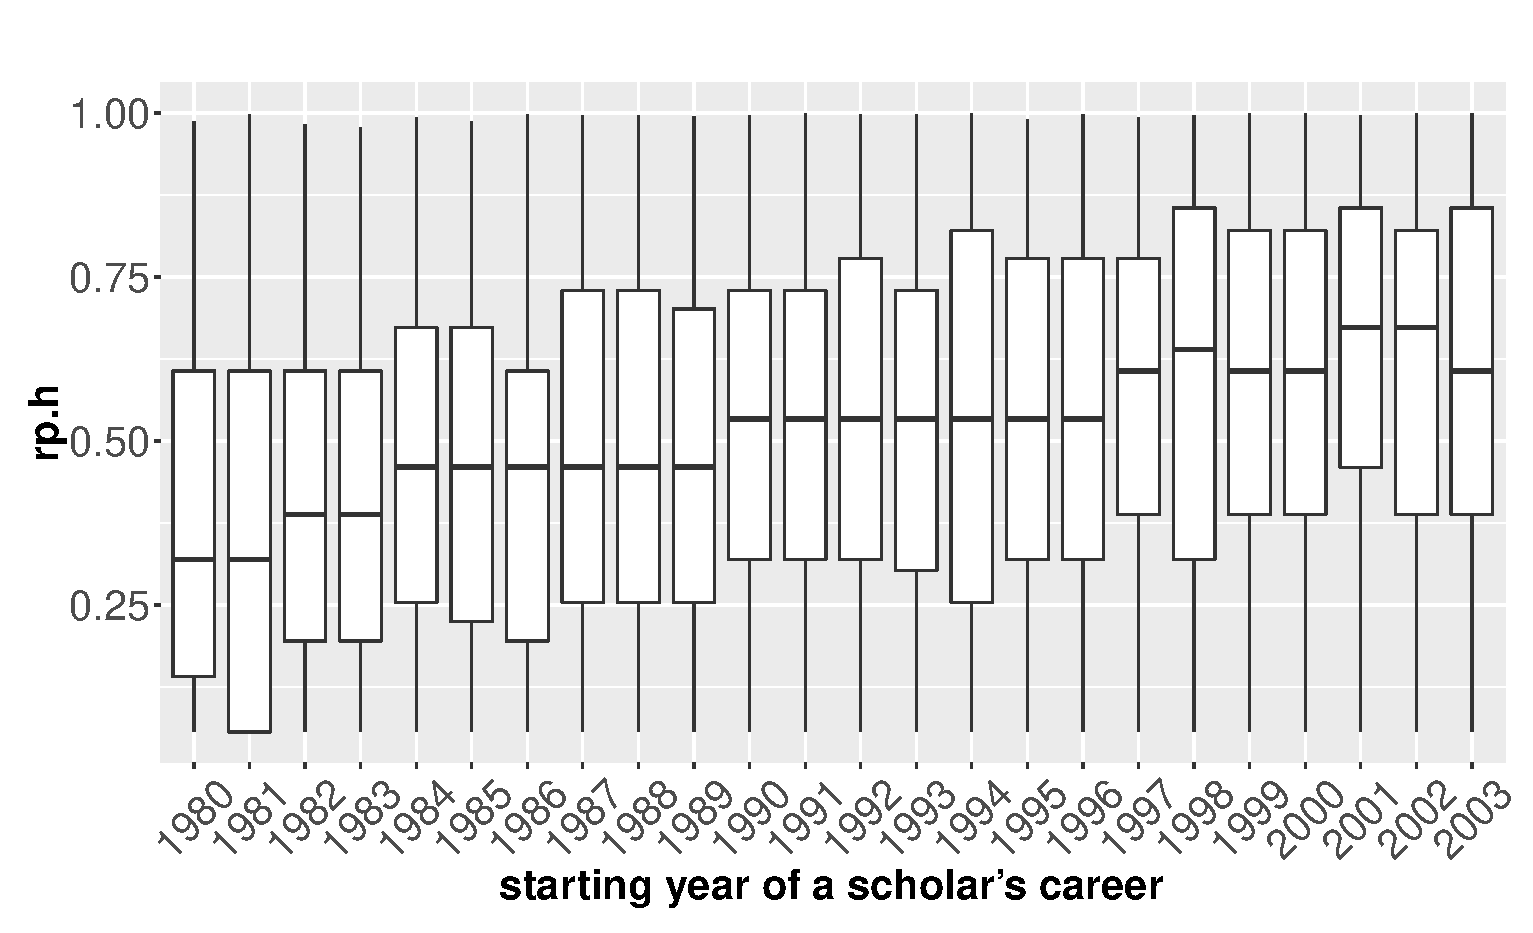
\includegraphics[width=\textwidth]{figures/exploratory/rph_age10.eps}
         \caption{rp.h$_{i10}$}
     \end{subfigure}
      \hfill
      \begin{subfigure}[b]{0.48\textwidth}
         \centering
         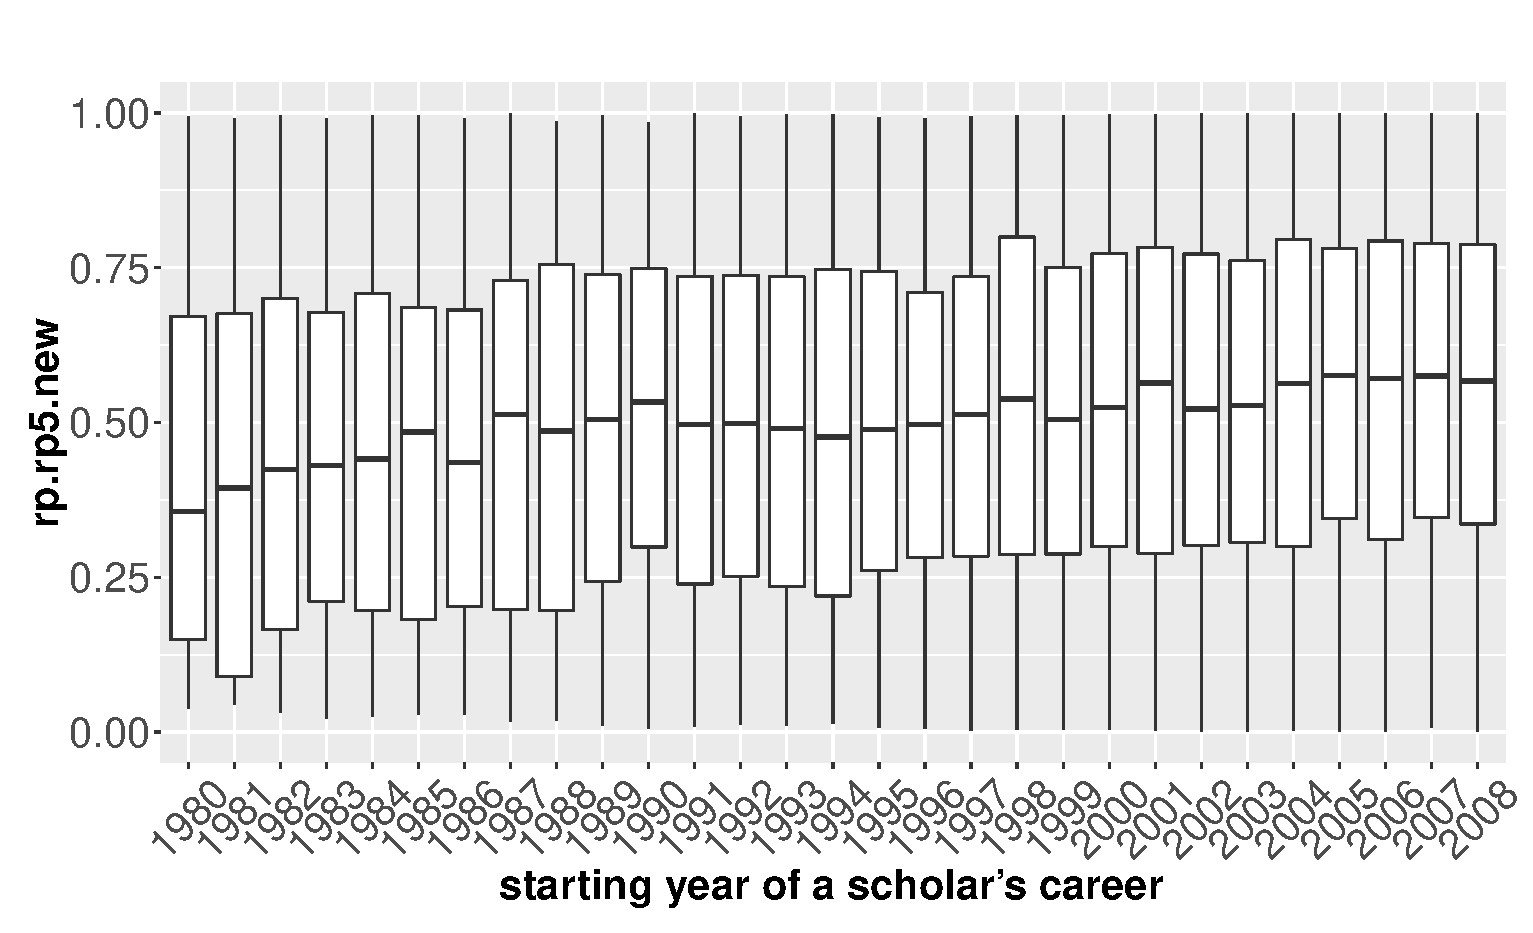
\includegraphics[width=\textwidth]{figures/exploratory/rprp5new_age5.eps}
         \caption{rp.rp5$_{i5}$}
     \end{subfigure}
     \hfill
     \begin{subfigure}[b]{0.48\textwidth}
         \centering
         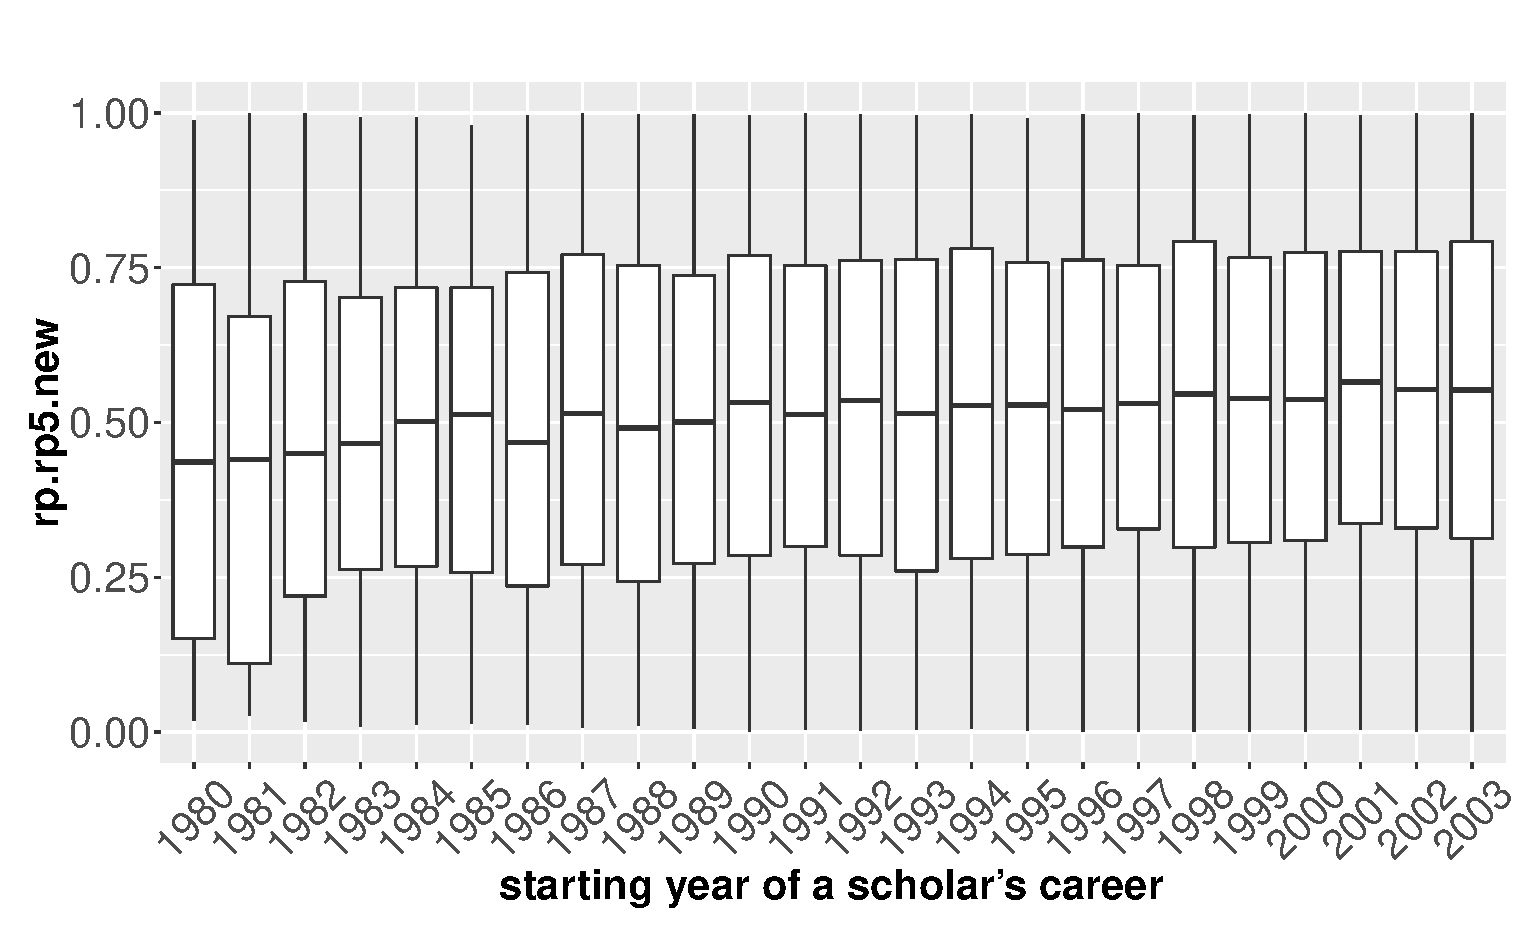
\includegraphics[width=\textwidth]{figures/exploratory/rprp5new_age10.eps}
         \caption{rp.rp5$_{i10}$}
     \end{subfigure}
    \caption{Different types of rank percentile indicators for scholars. rp.rp5 is stationary, while the other two are not.}
    \label{fig:compare_autrp}
\end{figure}

\fi

\end{refsection}